\documentclass{article}
\usepackage{hyperref}
\usepackage[ngerman]{babel}
\usepackage{amsmath}
\usepackage{amsfonts}
\usepackage{amsthm}
\usepackage{tcolorbox}
\usepackage[a4paper, total={7in, 9in}]{geometry}
\usepackage[font={scriptsize,it}]{caption}
\usepackage{scrextend}
\usepackage{graphicx}
\usepackage{caption}
\usepackage{subcaption}
\usepackage[utf8]{inputenc}
\usepackage[T1]{fontenc}
\DeclareUnicodeCharacter{2212}{-}

% floating figure for column
\newenvironment{Figure}
	{\par\medskip\noindent\minipage{\linewidth}}
	{\endminipage\par\medskip}

\theoremstyle{satz}
\newtheorem*{satz}{Satz}

\theoremstyle{definition}
\newtheorem{definition}{Definition}


\begin{document}
\begin{titlepage}
   \vspace*{\stretch{1.0}}
   \begin{center}
      \Large\textbf{Numerik 2 - HS19}\\
      \large\textit{Pascal Brunner - brunnpa7}
   \end{center}
   \vspace*{\stretch{2.0}}
\end{titlepage}


\tableofcontents
\newpage



\section{numerische Differationen}
Einleitender Text

\subsection{Lernziele}

\begin{description}
	\item{Sie können mittels Differenzenformeln die Ableitung einer Funktion numerisch annähern und die dabei gemachten Fehler qualifzieren und mit dem Satz von Taylor auch quantifzieren}
	\item{Sie können diese Differenzenformeln extrapoliere}
	\item{Sie kennen die wichtigsten Verfahren der numerischen Integration und können damit bestimmte Integrale berechnen. Sie können die dabei auftretenden Fehler bestimmen}
	\item{Sie können die Romberg-Extrapolation anwenden}
	\item{Sie können die hier vorgestellten Verfahren in MATLAB implentieren}
\end{description}

\subsection{Problemstellung}
Liegt die Funktion in Form einer differenzierbaren Funktionsgleichung y = f(x) vor, kann die Ableitung y' = f(x) analytisch mit den Verfahren der Analysis berechnet werden. Ist dies mit einem gewissen Aufwand verbunden, kann es sinnvoller sein, eine nummerische Näherung für die Ableitung zu verwenden. \\ \\Liegt die Funktion als eine Tabelle diskreter Funktionswerte (x\textsubscript{i},f(x\textsubscript{i})) mit i = 1,...,m vor, kann die Ableitung nicht analytisch berechnet werden. Dies ist beispielsweise bei realen Daten der Fall.\\ Dabei gibt es dann zwei Optionen:
	\begin{enumerate}
		\item{Zuerst werden die Wertpaare durch einen sogenannten Fit angenähert. Dadurch erhält man 		näherungsweise die Funktionsgleichung y = \~f(x). Der Vorteil dabei ist, dass der Einfluss von Fehlern und Ausreissern reduziert werden kann.  Danach wird die Funktionsgleichung y = \~f(x) entweder analytisch oder numerisch abgeleitet.}
		\item{Man verzichtet auf einen Fit und wendet direkt das numerische Verfahren an. Je nach Datenqualität und dem verwendeten Verfahren kann dies zu erheblichen Fehler führen}
	\end{enumerate}

\subsection{Repetition Taylor-Reihe}
Mit den Taylor-Reihen erhält man eine Näherung einer Funktion. Ziel dabei ist es das Taylor-Polynom n-ten Grades zu bestimmen, welches mit der Ableitung der Funktion n-ten Grades übereinstimmt. 
	\theoremstyle{definition}
	\begin{definition}[Allgemeine Formel zum Taylorpolynom]
		\begin{equation}
			T\textsubscript{n}f(x) = \sum\limits_{k=0}^{n} \frac{f^{(k)}(x)}{k!}x\textsuperscript{k}
		\end{equation}
	\end{definition}

\subsection{Vorwärtsdifferenz}
Wir gehen davon aus, dass wir es mit einer stetig differenzierbaren Funktion f\{a,b\} $\rightarrow$ $\mathbb{R}$ zu tun haben mit einem beliebigen x\textsubscript{0} $\in$ [a,b]. 
Gesucht sind Näherungswerte für die erste Ableitung $f'(x\textsubscript{0})$ oder auch für die k-te Ableitung $f^{(k)}(x\textsubscript{0})$. \\Dabei ist die (erste) 
Ableitung definiert als

\begin{equation} \label{eq1}
\begin{split}
f'(x\textsubscript{0}) & = \lim_{h \to 0} \frac{f(x\textsubscript{0} + h) - f(x\textsubscript{0})}{h} \\
 & \approx \frac{f(x\textsubscript{0} + h) - f(x\textsubscript{0})}{h} =: D\textsubscript{1}f(x\textsubscript{i},h)
\end{split}
\end{equation}

Man nennt $D\textsubscript{1}f(x\textsubscript{i},h)$ eine \textit{Vorwärtsdifferenz} (oder auch Differenzformel oder finite Differenz erster Ordnung), da sie einen Näherungswert für die erste Ableitung f'(x\textsubscript{0}) liefert, sofern h $\in$ $\mathbb{R}$ \dq ausreichend\dq  klein ist. 

Für eine stetige Funktion $f(x)$ kann \textit{h} beliebig kleine Werte annehmen und $f(x\textsubscript{0}+h)$ ist berechenbar. Der Einfachheitshalber machen wir die Einschränkung, dass \textit{h} konstant ist. Es gilt dabei $x\textsubscript{i+1} = x\textsubscript{i}+h$:\\
$D\textsubscript{1}f(x\textsubscript{i},h)= \frac{f(x\textsubscript{i} + h)-f(x\textsubscript{i})}{h}$ = $\frac{f(x\textsubscript{i} + h)-f(x\textsubscript{i})}{x\textsubscript{i+1}-x\textsubscript{i}}$

\theoremstyle{satz}
\begin{tcolorbox}

\begin{satz}[Taylor-Entwicklung]
Die Funktion f : [a,b] $\rightarrow$ $\mathbb{R}$ sei (n+1)-mal stetig differenzierbar, x\textsubscript{0} $\in$ [a,b]. Dann gibt es für alle x $\in$ [a,b] ein z zwischen x\textsubscript{0} und x, so dass
\begin{equation}
f(x) =  \sum\limits_{k=0}^{n} \frac{f\textsuperscript{(k)}(x\textsubscript{0})}{k!}(x-x\textsubscript{0})^k + R\textsubscript{n+1}(x) \\
\end{equation}
mit dem Taylorschen Restglied
\begin{equation}
R\textsubscript{n+1}(x) = \frac{f^{(n+1)}(z)}{(n+1)!}(x-x\textsubscript{0})^n+1
\end{equation}
\end{satz}
\end{tcolorbox}
Wir können f(x) mittels $x = x\textsubscript{0} + h$ bzw. $h = x - x\textsubscript{0}$ wie folgt schreiben:
\begin{equation}
f(x) = f(x\textsubscript{0}+h) = f(x\textsubscript{0})+f'(x\textsubscript{0})h + \frac{f''(x\textsubscript{0})}{2!}h^2+\frac{f'''(x\textsubscript{0})}{3!}h^3+\frac{f^(4)(x\textsubscript{0})}{4!}+...+\frac{f^(n+1)(z)}{(n+1)!}h^n+1
\end{equation}

\subsection{Diskretisierungsfehler}
Für die erste Ableitung (n=1) folgt durch umformen für den Fehler die Differenz erster Ordnung.
\begin{equation}
D\textsubscript{1}f(x\textsubscript{0},h)-f'(x\textsubscript{0}) = \frac{f''(z)}{2}h
\end{equation}
Den Fehler einer Differenzformel lässt sich allgemein beschreiben:
\theoremstyle{definition}
\begin{definition}[Diskretisierungsfehler / Fehlerordnung]
\item{Sei Df(x\textsubscript{0},h) eine Differenzformel für die Näherung von $f'(x\textsubscript{0})$. Dann bezeichnet man den absoluten Fehler
\begin{equation}
| Df(x\textsubscript{0},h) - f'(x\textsubscript{0})|
\end{equation}
als \textbf{Diskretisierungsfehler}}
\item{Die Differenzformel Df(x\textsubscript{0},h) hat die \textbf{Fehlerordnung} (oder kurz: Ordnung) k, falls es ein C > 0 gibt, so dass für genügend kleines h gilt:
\begin{equation}
|Df(x\textsubscript{0},h)-f'(x\textsubscript{0})| \leq C * h^k
\end{equation}
}
\end{definition}
\textbf{Bemerkung} \\ die obige Definition lässt sich auf Differenzformeln höhere Ableitungen anwenden \\ Man bezeichnet Ausdrücke, die für genügend kleines h durch Ch\textsuperscript{k} beschränktwerden, auch mit O(h\textsuperscript{k}) und man schreibt 
\begin{equation}
|Df(x\textsubscript{0},h)-f'(x\textsubscript{0})| = O(h^k)
\end{equation}

\subsection{zentrale Differenz}
Die zentrale Differenz hat zum Ziele eine genauere Differenzformel als D\textsubscript{1}f für die erste Ableitung zu berechnen. $\rightarrow$ wir möchten eine höhere Fehlerordnung erzielen. \\
Dabei verwenden wir x = x\textsubscript{0} $\pm$ h und n = 3 und setzen diese in die Taylorsche Formel ein:
\begin{equation}
\begin{split}
f(x\textsubscript{0} + h) & = f(x\textsubscript{0}) + f'(x\textsubscript{0})h + \frac{f''(x\textsubscript{0})}{2}h^2+\frac{f'''(x\textsubscript{0})}{6}h^3+\frac{f\textsuperscript{(4)}(z\textsubscript{1})}{24}h^4 \\
f(x\textsubscript{0} - h) & = f(x\textsubscript{0}) - f'(x\textsubscript{0})h + \frac{f''(x\textsubscript{0})}{2}h^2-\frac{f'''(x\textsubscript{0})}{6}h^3+\frac{f\textsuperscript{(4)}(z\textsubscript{1})}{24}h^4
\end{split}
\end{equation}
Durch subtrahieren der beiden Ausdrücke erhält man:
\begin{equation}
\begin{split}
f(x\textsubscript{0}+h)-f(x\textsubscript{0}-h) & = 2f'(x\textsubscript{0})h+\frac{f'''(x\textsubscript{0})}{3}h^3+... \\
\Rightarrow f'(x\textsubscript{0}) & = \frac{f(x\textsubscript{0}+h)-f(x\textsubscript{0}-h)}{2h}-\frac{f'''(x\textsubscript{0})}{6}h^2+...
\end{split}
\end{equation}
Also Resultat erhalten wir die zentrale Differenz D\textsubscript{2}f(x\textsubscript{0},h) als Näherung für $f'(x\textsubscript{0})$
\begin{equation}
D\textsubscript{2}f(x\textsubscript{0},h) = \frac{f(x\textsubscript{0}+h)-f(x\textsubscript{0}-h)}{2h}
\end{equation}
mit dem Diskretisierungsfehler der Fehlerordnung O(h\textsuperscript{2}):
\begin{equation}
|D\textsubscript{2}f(x\textsubscript{0},h)-f'(x\textsubscript{0})| = \frac{|f'''(x\textsubscript{0})|}{6}h^2+...
\end{equation}

\subsection{Rückwärtsdifferenz}
Analog zur Vorwärtsdifferenz bestimmen wir die Rückwärtsdifferenz mit der Fehlerordnung O(h)
\begin{equation}
D\textsubscript{3}f(x\textsubscript{0},h) = \frac{f(x\textsubscript{0}) - f(x\textsubscript{0}-h)}{h}
\end{equation}

\subsection{Vorwärtsdifferenz / zentrale Differenz / Rückwärtsdifferenz}
\begin{equation}
\begin{split}
D\textsubscript{1}f(x\textsubscript{0},h) & = \frac{f(x\textsubscript{0}+h)-f(x\textsubscript{0})}{h}\\
D\textsubscript{2}f(x\textsubscript{0},h) & = \frac{f(x\textsubscript{0}+h)-f(x\textsubscript{0} -h)}{2h}\\
D\textsubscript{3}f(x\textsubscript{0},h) & = \frac{f(x\textsubscript{0})-f(x\textsubscript{0}-h)}{h}
\end{split}
\end{equation}

\begin{Figure}
\centering
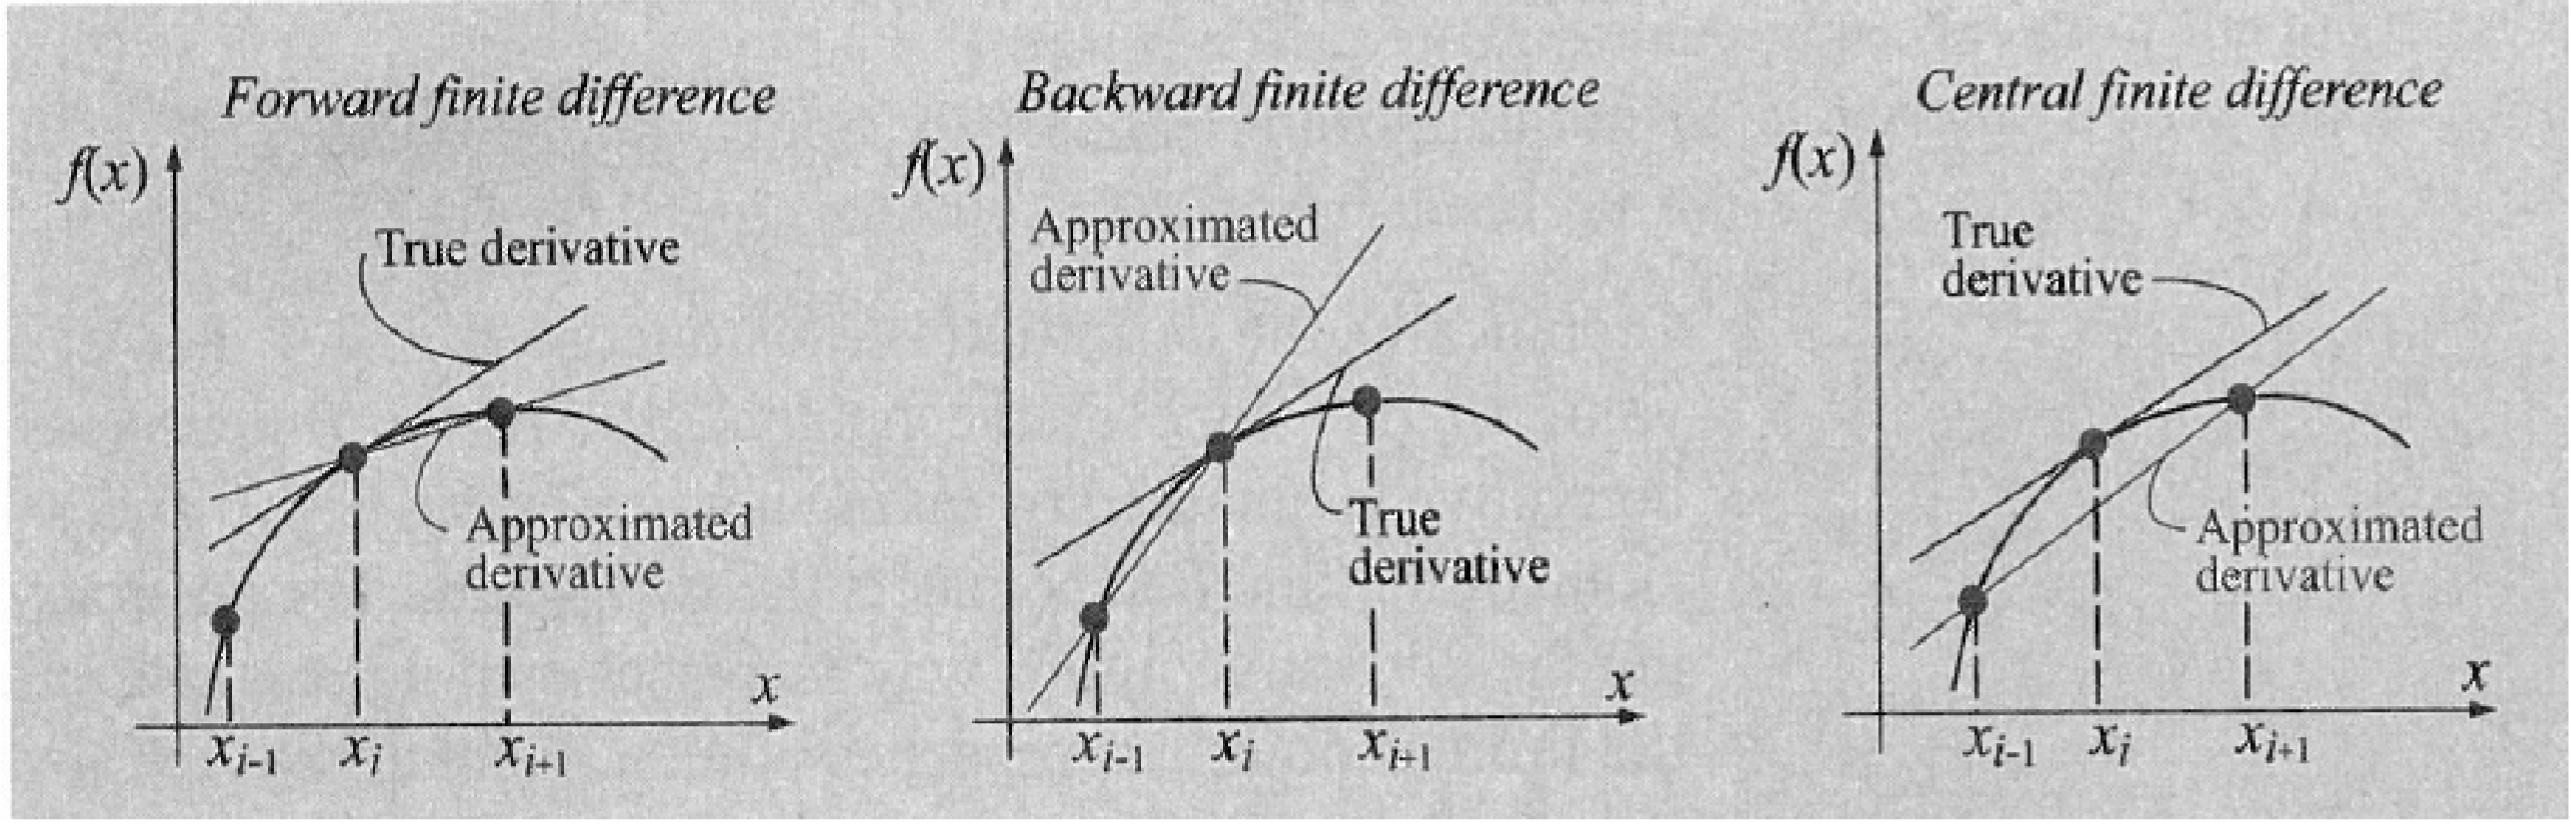
\includegraphics[width=500px]{img/vorwaerts_rueckwaerts_zentral_differenz.png}
	\captionof{figure}{Vorwärtsdiferenz (links), Rückwärtsdiferenz (Mitte) und zentrale Diferenz (rechts) als Näherung für die Ableitung $f'(xi)$}
	\label{fig:Vorwärtsdiferenz (links), Rückwärtsdiferenz (Mitte) und zentrale Diferenz (rechts) als Näherung für die Ableitung $f'(xi)$}
\end{Figure}

\subsection{Differenzformeln für höhere Ableitungen}
Analog zur ersten Ableitung kann die Differenzform als Näherung für die zweite Ableitung konstruiert werden (Vorwärtsdifferenz, zentrale Differenz, Rückwärtsdifferenz)
\begin{equation}
\begin{split}
D\textsubscript{4}f(x\textsubscript{0},h) & = \frac{f(x\textsubscript{0}+2h)-2f(x\textsubscript{0+h})+f(x\textsubscript{0})}{h^2}\\
D\textsubscript{5}f(x\textsubscript{0},h) & = \frac{f(x\textsubscript{0}+h)-2f(x\textsubscript{0})+f(x\textsubscript{0}-h)}{h^2}\\
D\textsubscript{6}f(x\textsubscript{0},h) & = \frac{f(x\textsubscript{0})-2f(x\textsubscript{0}-h)+f(x\textsubscript{0}-2h)}{h^2}
\end{split}
\end{equation}

\subsection{Differenzformeln für partielle Ableitungen}
Wenn es eine Funktion mit mehreren Variablen (bspw. u = u(x,y) ist, so verwendet man die partielle Ableitung. Dabei ergibt sich die erste Ableitung für x folgt:
\begin{equation}
\begin{split}
D\textsubscript{1}: \frac{\partial u}{\partial x}(x\textsubscript{0},y\textsubscript{0}) & \approx \frac{u(x\textsubscript{0}+h, y\textsubscript{0})-u(x\textsubscript{0}, y\textsubscript{0})}{h}\\
D\textsubscript{2}: \frac{\partial u}{\partial x}(x\textsubscript{0},y\textsubscript{0}) & \approx \frac{u(x\textsubscript{0}+h, y\textsubscript{0})-u(x\textsubscript{0}-h, y\textsubscript{0})}{2h}\\
D\textsubscript{3}: \frac{\partial u}{\partial x}(x\textsubscript{0},y\textsubscript{0}) & \approx \frac{u(x\textsubscript{0}, y\textsubscript{0})-u(x\textsubscript{0}-h, y\textsubscript{0})}{h}
\end{split}
\end{equation}

zweite partielle Ableitung nach x:
\begin{equation}
\begin{split}
D\textsubscript{4}: \frac{\partial ^2 u}{\partial x^2}(x\textsubscript{0},y\textsubscript{0}) & \approx \frac{u(x\textsubscript{0}+2h, y\textsubscript{0})-2u(x\textsubscript{0}+h,y\textsubscript{0})+u(x\textsubscript{0},y\textsubscript{0})}{h^2}\\
D\textsubscript{5}: \frac{\partial ^2 u}{\partial x^2}(x\textsubscript{0},y\textsubscript{0}) & \approx \frac{u(x\textsubscript{0}+h, y\textsubscript{0})-2u(x\textsubscript{0},y\textsubscript{0})+u(x\textsubscript{0}-h,y\textsubscript{0})}{h^2}\\
D\textsubscript{6}: \frac{\partial ^2 u}{\partial x^2}(x\textsubscript{0},y\textsubscript{0}) & \approx \frac{u(x\textsubscript{0}, y\textsubscript{0})-2u(x\textsubscript{0}-h,y\textsubscript{0})+u(x\textsubscript{0}-2h,y\textsubscript{0})}{h^2}
\end{split}
\end{equation}
$\rightarrow$ Analog geht man für die partielle Ableitung nach y vor.

\subsection{Extrapolation von Differenzformeln}
Erkenntnis von oben: höhere Ordnungen sind i.d.R. genauer als niederer Ordnung. Unter dem Begriff \textbf{Extrapolation} versteht man eine rekursive Methode, wo man aus einer Formeln niederer Ordnung Formeln höherer Ordnung gewinnen kann. 

\begin{tcolorbox}
\textbf{Algorithmus zur h-Extrapolation}
Sei D(h) eine Formel zur Näherung von $\bar{D}$ mit der Fehlerentwicklung
\begin{equation}
D(h)-D = c\textsubscript{1}h\textsuperscript{1}+c\textsubscript{2}h\textsuperscript{2}+c\textsubscript{3}h\textsuperscript{3}+...
\end{equation}
sei h grösser 0 eine Ausgangsschrittweite und D\textsubscript{i0} = D($\frac{h}{2\textsuperscript{i}})$ für i = 0,1, ..., m

Dann sind durch die Rekursion
\begin{equation}
D\textsubscript{ik}=\frac{2^k * D\textsubscript{i+1,k-1}-D\textsubscript{i,k-1}}{2^k -1}
\end{equation}
(Wobei k=1,2,...,m und i=0,1,...,m-k) Näherungen für $\bar{D}$ gegeben mit der Fehlerordnung k+1
\end{tcolorbox}

\begin{Figure}
\centering
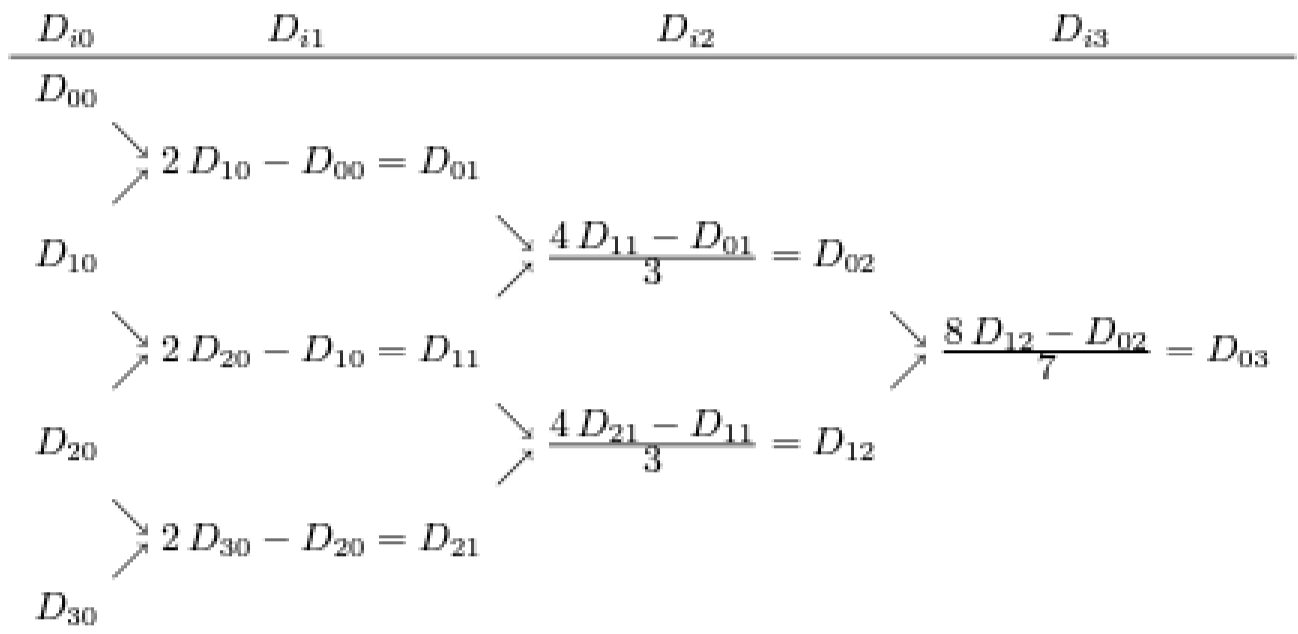
\includegraphics[width=200px]{img/Schema_h_Extrapolation.png}
	\captionof{figure}{Schema h-Extrapolation}
	\label{fig:Schema h-Extrapolation}
\end{Figure}

Wenn eine Differenzenformel eine Fehlerentwicklung mit nur geraden Potenzen hat, lässt sich die Extrapolation noch effizienter berechnen:
\begin{tcolorbox}
\textbf{Algorithmus zur h\textsuperscript{2}-Extrapolation}
Sei D(h) eine Formel zur Näherung von D mit der Fehlerentwicklung
\begin{equation}
D(h)-D = c\textsubscript{1}h\textsuperscript{2}+c\textsubscript{2}h\textsuperscript{4}+c\textsubscript{3}h\textsuperscript{6}+...
\end{equation}
sei h grösser 0 eine Ausgangsschrittweite und D\textsubscript{i0} = D($\frac{h}{2\textsuperscript{i}})$ für i = 0,1, ..., m

Dann sind durch die Rekursion
\begin{equation}
D\textsubscript{ik}=\frac{4^k * D\textsubscript{i+1,k-1}-D\textsubscript{i,k-1}}{4^k -1}
\end{equation}
(Wobei k=1,2,...,m und i=0,1,...,m-k) Näherungen für $\bar{D}$ gegeben mit der Fehlerordnung 2(k+1)
\end{tcolorbox}
\begin{Figure}
\centering
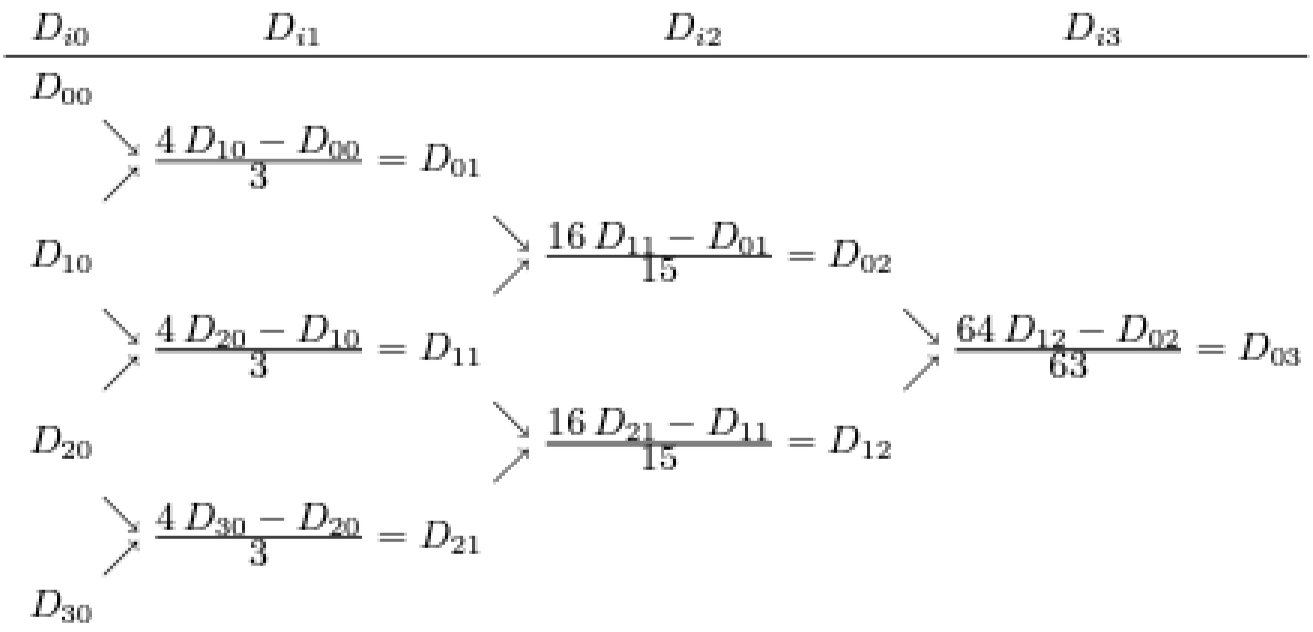
\includegraphics[width=200px]{img/Schema_h2_Extrapolation.png}
	\captionof{figure}{Schema $h^2$-Extrapolation}
	\label{fig:Schema $h^2$-Extrapolation}
\end{Figure}

\section{Numerische Integration}
Das Verfahren für die numerische Integration (auch Quadratur genannt) wird zum Lösen von nicht differenzierbaren Funktionen verwendet. 

\subsection{Problemstellung}
Für eine Funktion $f: \mathbb{R} \rightarrow 	\mathbb{R}$ soll das bestimmte Integral $I(f) = \int\limits_{b}^{a} f(x)dx$ auf einem Intervall \[a,b\] numerisch berechnet werden.

\begin{tcolorbox}
\textbf{Allgemeine Form der Quadraturverfahren}
\begin{equation}
I(f) = \sum\limits_{i=1}^{n}a\textsubscript{i}f(x\textsubscript{i})
\end{equation}
Dabei nennt man die x\textsubscript{i} die \textit{Stützstellen} oder \textit{Knoten} der Quadraturformel und die \textit{a\textsubscript{i}} die \textsubscript{Gewicht}. Die Funktion selbst kann wieder als Funktionsgleichung y=f(x) oder als Werttabelle (x\textsubscript{i}, f(x\textsubscript{i})) mit i = 1, ...,m vorliegen
\end{tcolorbox}

\subsection{Rechteck- und Trapezregel}
\theoremstyle{definition}
\begin{definition}[Rechteckregel / Trapezregel]
Die \textbf{Reckteckregel} (bzw. Mittelpunktregel $Rf$ und die \textbf{Trapezregel} $Tf$ zur Approximation von $\int\limits_{a}^{b} f(x)dx$ sind definiert als
\begin{equation}
\begin{split}
Rf & = f(\frac{a+b}{2})*(b-a)\\
Tf & = \frac{f(a) + f(b)}{2}*(b-a)
\end{split}
\end{equation}
\begin{itemize}

\item Wir erhalten die \textbf{Recktecksregel} wenn wir $f(x)$ in $\int\limits_{a}^{b}dx$ durch eine Konstante (Polynom 0. Grades) ersetzten.
\item Wenn wir $f(x)$ durch eine Gerade (Polynom 1. Grades) ersetzen, erhalten wir analog die \textbf{Trapezregel}
\end{itemize}
\end{definition}

\begin{Figure}
\centering
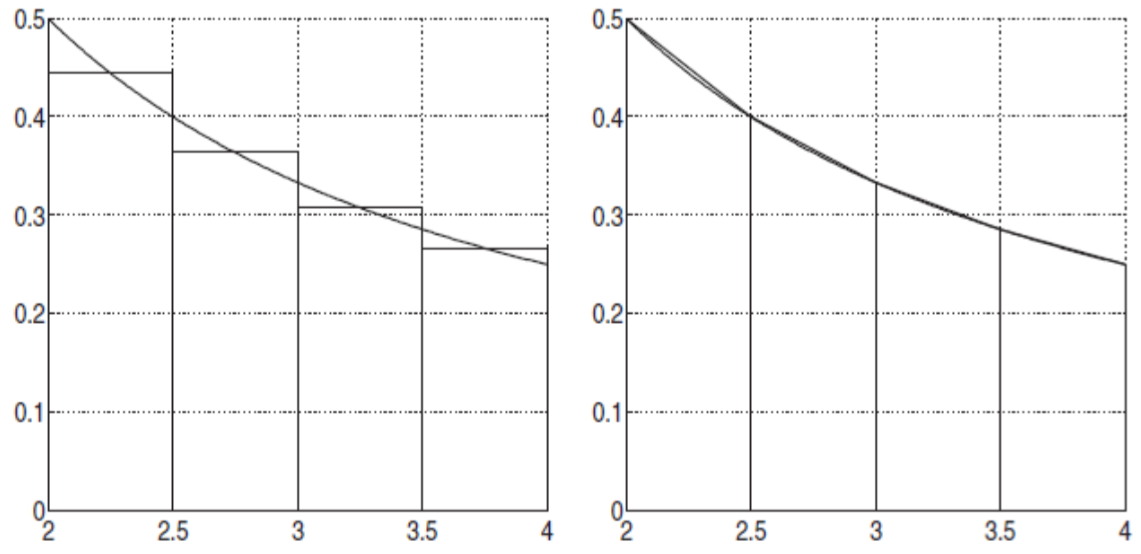
\includegraphics[width=200px]{img/sumRechteckregel_sumTrapezregel.png}
	\captionof{figure}{(links)summierte Rechtecksregel, (rechts) summierte Trapezregel}
	\label{fig:(links)summierte Rechtecksregel, (rechts) summierte Trapezregel}
\end{Figure}

Um die Genauigkeit zu Steigern, lohnt sich das Intervall \[a,b\] in \textit{n} Subintervalle mit der Schrittweite $h=\frac{b-a}{n}$ zu unterteilen und anschliessend aufzusummieren. Als Resultat erhalten wir die summierten Regeln.

\theoremstyle{definition}
\begin{definition}[summierte Rechteckregel / summierte Trapezregel]
Sei $f: [a,b] \rightarrow \mathbb{R}$ stetig, n $\in \mathbb{N}$ die Anzahl Subintervalle \[x\textsubscript{i}, x\textsubscript{i+1}\] auf \[a,b\] mit der konstanten Breite $h=x\textsubscript{i+1} - x\textsubscript{i} = \frac{b-a}{n}$ und $x\textsubscript{i} = a + i * h$ für i = 0, ..., n-1.\\
Die \textbf{summierte Rechteckregel} (bzw. summierte Mittelpunktregel) $Rf(h)$ und die \textbf{summierte Trapezregel} $Tf(h)$ zur Approximation von $\int\limits_{a}^{b} f(x)dx$ sind gegeben durch
\begin{equation}
\begin{split}
Rf(h) & = h * \sum\limits_{i=0}^{n-1}\\
Tf(h) & = h*(\frac{f(a)+f(b)}{2}+\sum\limits_{i=1}^{n-1}f(x\textsubscript{i}))
\end{split}
\end{equation}
\end{definition}

\subsection{Die Simpson-Regel}
Wenn wir $f(x)$ durch ein Polynom $p(x)$ 2. Grades ersetzen erhalten wir einen neuen Ansatz:\\
Wir machen für $p(x)$ und $x \in [a,b]$ den Ansatz
\begin{equation}
p(x) = \alpha + \beta(x-a) + \gamma(x-a)(x-b)
\end{equation}
\begin{Figure}
\centering
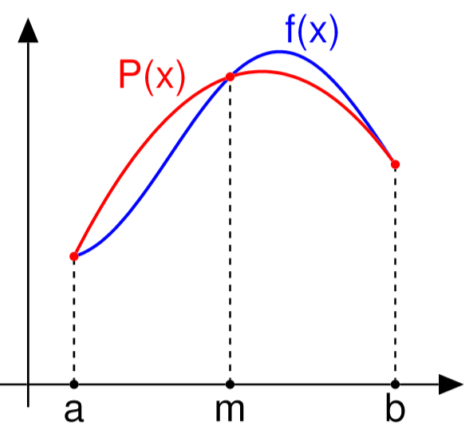
\includegraphics[width=100px]{img/SimpsonRegel.png}
	\captionof{figure}{Funktion f(x) wird auf dem Intervall durch ein Polynom P(x) angenähert}
	\label{fig:Funktion f(x) wird auf dem Intervall durch ein Polynom P(x) angenähert}
\end{Figure}
und fordern, dass p(x) an den Stellen $x=a$, $x=\frac{b+a}{2}$ und $x3=b$ exakt mit f(x) übereinstimmt, also:
\begin{equation}
\begin{split}
p(a) &= \alpha != f(a)\\
p(\frac{b+a}{2}) &= \alpha + \beta(\frac{b+a}{2}-a) + \gamma(\frac{b+a}{2}-a)(\frac{b+a}{2}-b) = \alpha + \beta(\frac{b-a}{2}) + \gamma(\frac{b-a}{2})(\frac{a-b}{2}) != f(\frac{b+a}{2})\\
p(b) &= \alpha + \beta(b-a) != f(b)
\end{split}
\end{equation}
Dabei ist die Schrittweite mittels $h = \frac{b-a}{2}$ gesetzt. Das Näherungspolynom $f(x)$ ist eindeutig bestimmt und es kann mittels der Potenzregel einfach integriert werden. da $f(x) \approx p(x)$ gilt: \\
\begin{tcolorbox}
\textbf{Simpson-Regel}
\begin{equation}
\int\limits_{a}^{b}f(x)dx\approx \int\limits_{a}^{b}p(x)dx = \frac{h}{3}(f(a)+4f(\frac{a+b}{2})+\frac{1}{2})+f(b))
\end{equation}
\end{tcolorbox}
Analog zur Rechtecks- und Trapez-Regel kann die Genauigkeit erhöht werden. Dies geschieht in dem wir das Intervall $[a,b]$ in \textit{n} Intervalle mit der Schrittweite $h=\frac{b-a}{n}$ unterteilt und aufsummiert wird.
\begin{tcolorbox}
\textbf{summierte Simpson-Regel}
\begin{equation}
Sf(h) = \frac{h}{3}(\frac{1}{2}+\sum\limits_{k=1}^{n-1}f(x_k)+2\sum\limits_{k=1}^{n}f(\frac{x_{k-1}+x_k}{2}+\frac{1}{2}f(b))
\end{equation}
wobei wir $x_k = a+k*h$ gesetzt haben
\end{tcolorbox}

\subsection{Der Fehler der summierten Quadraturformeln}
Der Fehler einer Näherung ist wie immer definiert als Betrag der Differenz zwischen dem exakten Wert und der Näherung. 
\theoremstyle{satz}
\begin{tcolorbox}
\begin{satz}[Fehlerabschätzung für summierte Quadraturformeln]
Wobei $Rf(h)$ für die summierte Reckeckregel, $Tf(h)$ für die summierte Trapezregel und $Sf(h)$ für die summierte Simpsonregel gilt:
\begin{equation}
\begin{split}
|\int\limits_a^{b}f(x)dx-Rf(h)| & \leq \frac{h^2}{24}(b-a) * max_{x\in[a,b]}|f''(x)|\\
|\int\limits_a^{b}f(x)dx-Tf(h)| & \leq \frac{h^2}{12}(b-a) * max_{x\in[a,b]}|f''(x)|\\
|\int\limits_a^{b}f(x)dx-Sf(h)| & \leq \frac{h^4}{2800}(b-a) * max_{x\in[a,b]}|f^{(4)}(x)|\\
\end{split}
\end{equation}
\end{satz}
\end{tcolorbox}

\subsection{Gauss-Formel}
Bis zum aktuell Zeitpunkt haben wir die Stützstellen jeweils $x_i$ äquidistant gewählt ($\rightarrow$ die Schrittweite $h=\frac{b-a}{n}$ war konstant) und konnten somit die Recktecks-, Trapez- und Simpson-Formel herleiten. Diese drei Formeln werden auch als Newton-Cotes Formeln der Ordnung \textit{N} = 0, 1 und 2 bezeichnet. Wobei dies dem Grad des verwendeten Polynomons entspricht.\\
Die Stützstellen $x_i$ können jedoch auch so gewählt werden, dass das Integral $\int\limits_{a}^{b}f(x)dx$ 'optimal' approximieren. Daraus erhält man die Gauss-Formel.\\
Dafür werden die Stützstellen $x_i$ und die Gewichte $a_i$ in der generellen Quadraturformel\\
\begin{equation}
I(f) = \sum\limits_{i=1}^{n}a_i f(x_i)
\end{equation}
so gewählt, dass die \textit{Fehlerordnung} möglichst hoch bzw. der Fehler \\
\begin{equation}
|\int\limits_{a}^{b}f(x)dx-I(f)|
\end{equation}
möglichst klein wird
\theoremstyle{satz}
\begin{tcolorbox}
\begin{satz}[Gauss-Formel für n = 1, 2, 3:]
Die Gauss-Formeln für n=1,2,3 für $\int\limits_{a}^{b}f(x)dx$ $\approx$ $\frac{b-a}{2}\sum\limits_{i=1}^{n}a_if(x_i)$ lauten:
\begin{equation}
\begin{split}
n=1:		G_1f &=(b-a)*f(\frac{b+a}{2})\\
n=2:		G_2f &=\frac{b-a}{2}[f(-\frac{1}{\sqrt{3}}*\frac{b-a}{2}+\frac{b+a}{2})+f(\frac{1}{\sqrt{3}}*\frac{b-a}{2}+\frac{b+a}{2})]\\
n=3:		G_3f &=\frac{b-a}{2}[\frac{5}{9}*f(-\sqrt{0.6}*\frac{b-a}{2}+\frac{b+a}{2})+\frac{8}{9}*f(\frac{b+a}{2})]\\
&+\frac{b-a}{2}[\frac{5}{9}*f(\sqrt{0.6}*\frac{b-a}{2}+\frac{b+a}{2})]
\end{split}
\end{equation}
\end{satz}
\end{tcolorbox}

\subsection{Romberg-Extrapolation}
Auch für die Integration gibt es einen Extrapolations-Ansatz, welcher erlaubt aus einigen Anfangsnäherungen für ein bestimmtes Integral einen genaueren Wert zu extrapolieren. Es kann das exakte Schemata des h- bzw. $h^2$ Algorithmus verwendet werden.
\textbf{Vorraussetzung} ist, dass wir aus der bekannten Quadraturformel entweder eine Fehlerentwicklung in h oder $h^2$ haben. $\rightarrow$ h gibt jeweils die Schrittweise an. Die Trapezformel hat eine Fehlerentwicklung in geraden Potenzen der Schrittweite. $\rightarrow$ der $h^2$-Algorithmus ist anwendbar.
\theoremstyle{satz}
\begin{tcolorbox}
\begin{satz}[Romberg-Extrapolation]
Für die summierte Trapezregel $Tf(h)$ zur näherungsweisen Berechnung von $I(f) = \int\limits_a^bf(x)dx$ gilt:\\
Sei $T_{i0} = Tf(\frac{b-a}{2^i})$ für i = 0, 1,...,m. Dann sind durch die Rekursion
\begin{equation}
T_{ik} = \frac{4^k*T_{i+1,k-1}-T_{i,k-1}}{4^k-1}
\end{equation}
für k = 1,2,...,m und i=0,1,...,m-k Näherungen der Fehlerordnung 2k+2 gegeben. Diese Methode heisst \textbf{Romberg-Extrapolation}. Die verwendete Schrittweitenfolge $h_i=\frac{b-a}{2^i}$ heisst auch \textbf{Romberg-Folge}
\end{satz}
\end{tcolorbox}
\textit{Erkenntnis:}\\
Man kann das Schema aus der Differation nochmals verwenden. Dafür berechnen wir die summierte Trapezformel für die Schrittweiten $h_i = \frac{b-a}{2^i}$ (i=0,1,2,...,m) $\rightarrow$ bspw. $h, \frac{h}{2}, \frac{h}{4},\frac{h}{8}$ (m=3). Daraus erhalten wir $T_{00},T_{10},T_{20},T_{30}$ und können anschliessend wieder extrapolieren. Dabei muss die Anzahl $n=2^i$ der Intervalle für die Berechnung von $T_{i0}$ angepasst werden.
\begin{Figure}
\centering
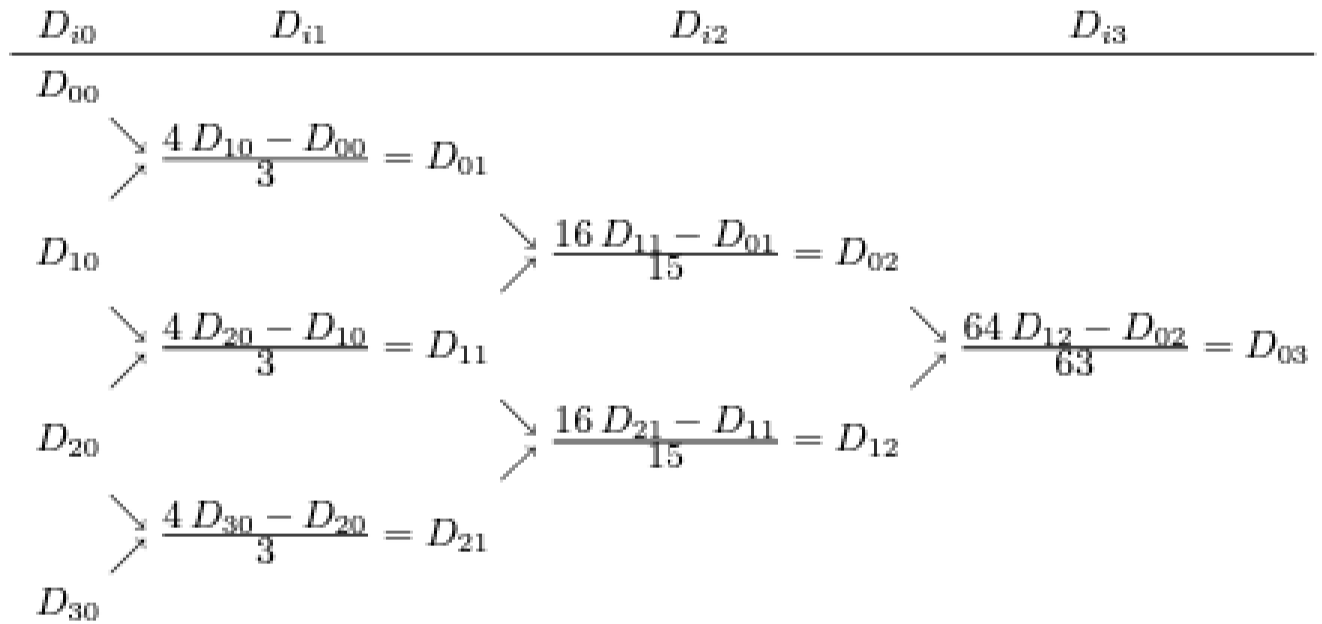
\includegraphics[width=200px]{img/RombergExtrapolation.png}
	\captionof{figure}{Schema für Romberg Extrapolation}
	\label{fig:Schema für Romberg Extrapolation}
\end{Figure}

\section{Einführung in gewöhnliche Differentialgleichungen}
Einleitender Text

\subsection{Lernziele}

\begin{description}
	\item{Sie kennen die Definitionen einer gewöhnlichen Differentialgleichung n-ter Ordnung und eines Anfangswertproblems}
	\item{Sie verstehen das Prinzip eines Richtungsfeldes und können Richtungsfelder interpretieren und zeichnen}
	\item{Sie können gewöhnliche Differentialgleichung lösen basierend auf dem Euler-Verfahren, dem modifizierten Euler-Verfahren, dem Mittelpunkt-Verfahren und den Runge-Kutta Verfahren}
	\item{Sie können die hier vorgestellten Mehrschrittverfahren anwenden}
	\item{Sie können Differentialgleichungen n-ter Ordnung in ein Sytem von n Differentialgleichungen 1. Ordnung umwandeln und dieses System lösen}
	\item{Sie kennen den Begriff Stabilität}
\end{description}
	
\subsection{Problemstellung}
In vielen Prozessen (bspw. Natur oder Technik) spielt die zeitliche Änderungen von beobachtenbaren Grösse $\rightarrow y(t)$ eine wichtige Rolle. Häufig ist die zeitliche Änderung einer solchen Grösse, also $\frac{dy}{dt}$, abhängig von der Grösse $y(t)$. D.h. wir können $\frac{dy}{dt}$ durch eine Funktion $f$ ausdrücken, die von der Zeit $t$ aber eben auch von der eigentlichen Grösse $y(t)$ abhängt:
\begin{equation}
\frac{dy}{dt} = f(t,y(t))
\end{equation}
$\rightarrow$ auch 'gewöhnliche Differentialgleichung 1. Ordnung' genannt. 1. Ordnung, da die erste Ableitung auftritt.
Beispiel hierfür wäre der radioaktiver Zerfall.

\begin{tcolorbox}
\begin{definition}[\textbf{Gewöhnliche Differentialgleichung (kurz:DGL) n-ter Ordnung}]
Eine Gleichung, in der Ableitungen einer unbekannten Funktion $y = y(x)$ bis zur n-ten Ordnung auftreten, heisst eine \textit{gewöhnliche Differentialgleichung n-ter Ordnung.} Sie hat die explizite Form
\begin{equation}
y^{(n)}(x)=f(x,y(x),y'(x), ...,y^{(n-1)}(x))
\end{equation}
Gesucht sind die Lösungen y = y(x) dieser Gleichung, wobei die Lösungen $y$ auf einem Intervall \[a, b\] definiert sein sollen, $y: [a,b] \rightarrow \mathbb{R}$
\end{definition}
\end{tcolorbox}

\begin{tcolorbox}
\begin{definition}[\textbf{Anfangswertproblem}]
Bei einem Anfangswertproblem für eine Differentialgleichung n-ter Ordnung werden die Lösungsfunktion $y=y(x)$ noch n Werte vorgeschrieben, nämlich der Funktionswert an einer bestimmten Stelle $x_0$ sowie die Werte der ersten n-1 Ableitungen an der gleichen Stelle.

\textit{Für die hier betrachteten Differentialgleichungen 1. und 2. Ordnung heisst das:}
\begin{itemize}
\item {\textit{Differentialgleichung 1. Ordnung:} Gesucht ist diejenige \textit{spezifische} Lösungskurve $y=y(x)$, die durch den vorgegebenen Punkt $P=(x_0,(y(x_0))$ verläuft.} 
\item {\textit{Differentialgleichung 2. Ordnung:} Gesucht ist diejenige \textit{spezifische} Lösungskurve $y=y(x)$ die durch den vorgegebenen Punkt $P = (x_0, y(x_0))$ verläuft und im Punkt $x_0$ die vorgegebenen Steigung $y'(x_0) = m$ besitzt.}
\end{itemize}
\end{definition}	
\end{tcolorbox}

\subsection{Richtungsfelder für Differentialgleichungen 1. Ordnung}
Die Differentialgleichung 1. Ordnung ihr Ihre Lösungen lassen sich mit Hilfe von sogenannten Richtungsfeldern veranschaulichen.\\
Ausgangspunkt ist die geometrische Interpretation der Gleichung:
\begin{equation}
y'(x) = f(x, y(x))
\end{equation}
Aus dieser Gleichung ist ersichtlich, dass es einen Zusammenhang zwischen der Steigung $y'(x)$, der gesuchten Funktion $y(x)$ für einen gegebenen Punkt x und dem Punkt $(x,y(x))$.\\
Wenn wir uns dies in einer $(x,y)$-Ebene veranschaulichen hat es folgende Auswirkung:\\
Wenn der Graph einer Lösung $y$ durch einen Punkt $(x,y)$ verläuft, so muss er dort die Steigung $y'$ haben. Dementsprechend können wir in der $(x,y)$-Ebene an einem belieben $(x,y)$-Punkt die Steigung $y'(x) = f(x, y(x))$ ausrechnen und durch einen kleinen Pfeil graphisch darstellen. Als Resultat erhalten wir mit all den Pfeilen zu jeden jeweiligen Punkten die Richtung der Lösungskurve.\\
$\rightarrow$ Dies wird auch Richtungsfeld der Differentialgleichung genannt. Dabei verlaufen die Lösungskurven der Gleichung stets tangential zu den Pfeilen im Richtungsfeld.
\begin{Figure}
\centering
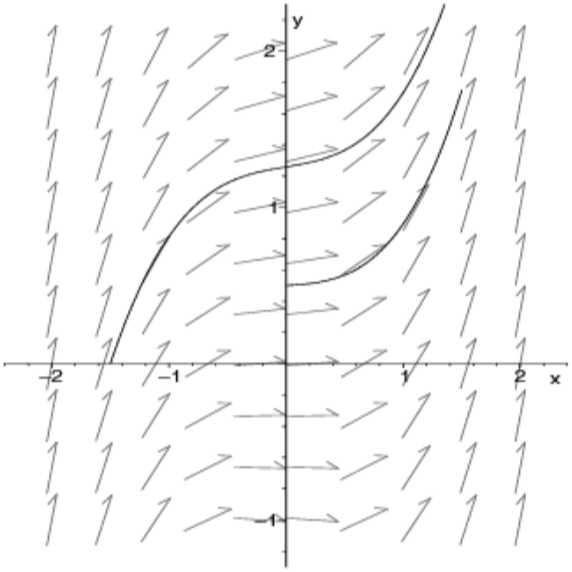
\includegraphics[width=200px]{img/BeispielRichtungsfeld.png}
	\captionof{figure}{Beispiel für ein Richtungsfeld für die Gleichung $y'(x)=f(x,y(x))=x^2+0.1*y(x)$}
	\label{fig:Beispiel für ein Richtungsfeld}
\end{Figure}
Die Idee vieler numerischer Verfahren zur Lösung von Anfangswertproblemen ist es nun, dem Richtungsfeld möglichst genau zu folgen. Jedoch besteht, dass Problem, dass ein solches Richtungsfeld aus unendlich vielen Punkten besteht. Damit man hier trotzdem zu einer Lösung kommt, braucht man eine \textit{Diskretisierung}.

\subsection{Das Euler-Verfahren}
Das einfachste numerische Einschrittsverfahren zur Lösung von Anfangswertproblem ist das klassische Euler-Verfahren. Jedoch hat es einige Einschränkungen und wird in der Praxis nicht wirklich verwendet. Verbesserte Verfahren sind das modifizierte Euler-Verfahren oder das Mittelpunkt-Verfahren, welche in den nächsten Kapitel behandelt werden.

\subsubsection{Das klassische Euler-Verfahren}
Wir gehen vom folgenden Anfangswertproblem aus:
\begin{equation}
\frac{dy}{dx} = f(x, y(x)) \textrm{ mit } y(a) = y_0
\end{equation}
Entsprechend ist $x_0 = a$ die einzige Stelle, welche wir exakt bestimmen können (da $y(x_0) = y_0$ vorgegeben ist.). Dies ist ebenfalls auch die einzige Stelle wo wir $y'$ exakt kennen $\rightarrow$ $y'(x_0) = f(x_0,y(x_0)) = f(x_0, y_0)$.\\
Dem Startpunkt $(x_0, y(x_0))$ hat entsprechend eine hohe Bedeutung, denn alle weiteren Werte werden Fehler enthalten, da wir dem Richtungsfeld nicht exakt folgen können.\\
Es wird angenommen, dass die Steigung in den Punkten um $(x_0, y(x_0))$ nur wenig von $y'(x_0)$ abweicht. \\
Wir können dann die Steigung der Sekanten durch die Punkte $(x_0,y(x_0))$ und $(x_1,y(x_1))$ mit der Steigung $y'(x_0)$ gleichsetzen und nach $y(x_1)$ auflösen:
\begin{equation}
y'(x_0) = f(x_0, y(x_0)) \approx \frac{y(x_1)-y(x_0)}{x_1 - x_0} = \underbrace{\frac{y(x_1)-y(x_0)}{h}}_{\substack{D_1 y(x_0,h)}} \Rightarrow x(x_1) \approx y(x_0)+h*f(x_0,y(x_0))=y_1
\end{equation}
Wir folgen sozusagen der Tangente im Punkt $(x_0, y(x_0))$ um die Schritte weite $h$ in der Hoffung, dass wir dann genügend nahe an den Punkt $y(x_1)$ rankommen. Dabei verwenden wir im Prinzip nichts anderes als die Vorwärtsdifferenz $D_1$.  Wenn die Schrittweite genügend klein ist, sollte auch der Fehler entsprechend klein sein und umgekehrt.\\
Dieser Schritt lässt sich nun ausgehend von der Näherung $y_1 \approx y(x_1)$ wiederholen, wir erhalten dann $y(x_2) \approx y_1+h*f(x_1, y_1) = y_2$ usw. 

\begin{tcolorbox}
\begin{definition}[\textbf{Algorithmus Euler-Verfahren}]
Gegeben sei für x $\in$ \[a,b\] das Anfangswertproblem:
\begin{equation}
y' = f(x,y) \textrm{ mit } y(a)=y_0
\end{equation}
Das Euler-Verfahren zur numerischen Lösung lautet:
\begin{equation}
\begin{split}
x_{i+1} &= x_i + h\\
y_{i+1} &= y_i + h * f(x_i, y_i)
\end{split}
\end{equation}
Wobei $x_0 = a, x_i = a+i*h$ für i=0, ..., n-1 $n \in\mathbb{N}$ und $h = \frac{b-a}{n}$ 
\end{definition}
\end{tcolorbox} 
\begin{Figure}
\centering
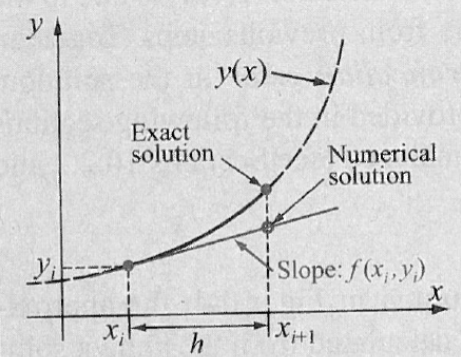
\includegraphics[width=200px]{img/KlassischeEulerVerfahren.png}
	\captionof{figure}{Euler-Verfahren zur Berechnung von $y_{i+1}$ an der Stelle $x_{i+1}$ basierend auf der Tangente mit der Steigung $f(x_i, y_i)$ an der Stelle $x_i$ }
	\label{fig:Beispiel für das klassische Euler-Verfahren}
\end{Figure}

\subsubsection{Das Mittelpunkt-Verfahren}
Das klassische Euler-Verfahren beruht darauf, die Steigung $y'(x_i)$ am Punkt $(x_i,y_i)$ zu berechnen und der Tangente in diesem Punkt eine Schrittweite $h$ zu folgen. Beim Mittelpunktverfahren folgt man der Tangente nur die halbe Schrittweite $\frac{h}{2}$ und berechnet beim Mittelpunkt des Intervalls $x_{\frac{h}{2}} = x_i + \frac{h}{2}$ die neue Steigung $y_{\frac{h}{2}}$:
\begin{equation}
y_{\frac{h}{2}} = y_i + \frac{h}{2}*f(x_i, y_i)
\end{equation}
Anschliessend geht man zurück an den Ausgangspunkt $(x_i, y_i)$ und benutzt die berechnete Steigung $y_{\frac{h}{2}}$ für einen ganzen Schritt der Schrittweite $h$.

\begin{tcolorbox}
\begin{definition}[\textbf{Algorithmus: Mittelpunkt-Verfahren}]
Gegeben sei für $x \in [a,b]$ das Anfangswertproblem
\begin{equation}
y' = f(x,y)  \textrm{ mit } y(a) = y_0
\end{equation}
Das Mittelpunktverfahren zur numerischen Lösung lautet:
\begin{equation}
\begin{split}
x_{\frac{h}{2}} &= x_i + \frac{h}{2}\\
y_{\frac{h}{2}} &= y_i + \frac{h}{2}*f(x_i, y_i)\\
x_{x+1} &= x_i + h\\
y_{x+1} &= y_i + h*f(x_{\frac{h}{2}},y_{\frac{h}{2}})
\end{split}
\end{equation}
Wobei $x_0 = a$, $x_i = a+i*h$ für i = 0,...,n-1 $(n \in \mathbb{N})$ und $h = \frac{b-a}{n}$
\end{definition}
\end{tcolorbox}
\textbf{Beispiel Mittelpunkt-Verfahren}\\
\textit{Wir berechnen die numerische Lösung des Anfangsproblems mit dem Mittelpunkt-Verfahren:
\begin{equation}
y'(t) = f(t,y(t)) = t^2+0.1*y(t)
\end{equation}
mit $y(-1.5)=0$ auf dem Intervall $[a,b] = [-1.5, 1.5]$ und n = 5
}
\begin{equation}
\begin{split}
n &= 5 \Rightarrow h = \frac{b-a}{n} = \frac{1.5-(-1.5)}{5} = 0.6\\
t_i &= a +ih = -1.5 + i*0.6   (i = 0, 1,..., 5)\\
y_{i+1} &= y_i + hf(t_{\frac{h}{2}},y_{\frac{h}{2}}) = y_i + h(t^2_{\frac{h}{2}} + 0.1y_{\frac{h}{2}})
\end{split}
\end{equation}
\begin{Figure}
\centering
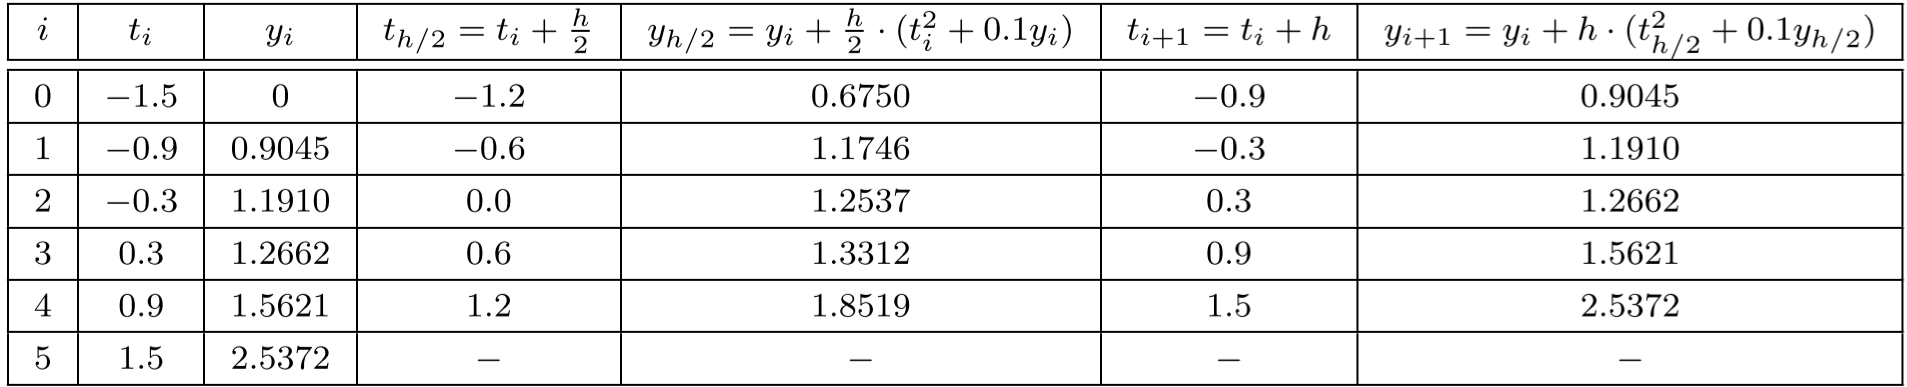
\includegraphics[width=500px]{img/MittelwertVerfahrenBeispiel.png}
	\captionof{figure}{Tabelle für das Mittelpunkt-Verfahren}
	\label{fig:Tabelle für das Mittelpunkt-Verfahren}
\end{Figure}

\subsubsection{Das modifizierte Euler-Verfahren (auch Heun-Verfahren genannt)}
Beim modifizierten Euler-Verfahren verwendet man den Durchschnitt zweier Steigungen.\\
Zuerst folgt man wie beim klassischen Euler-Verfahren ausgehend vom Punkt $(x_i, y_i)$ der Tangete der Steigung $f(x_i, y_i)$ einen ganzen Schritt und erhält den neuen Punkt $(x_{i+1}, y^{Euler}_{i+1})$ wobei $y^{Euler}_{i+1} = y_i+h*f(x_i,y_i)$. Anschliessend berechnet man im Punkt $(x_{i+1},y^{Euler}_{i+1})$ die nächste Steigung $f(x_{x+1}, y^{Euler}_{i+1})$. Danach wird der Durchschnitt der beiden Steigungen genommen und vom Ausgangspunkt $(x_i, y_i)$ ein Schritt mit Schrittlänge $h$ gemacht zum neuen Punkt $(x_{i+1}, y_{i+1})$.

\begin{tcolorbox}
\begin{definition}[\textbf{Algorithmus: Modifiziertes Euler-Verfahren}]
Gegeben sei für $x \in [a,b]$ das Anfangswertproblem
\begin{equation}
y' = f(x,y) \textrm{ mit } y(a) = y_0
\end{equation}
Das modifizierte Euler-Verfahren zur numerischen Lösung lautet:
\begin{itemize}
\item[a)]{Führe das klassische Euler-Verfahren durch und speichere die erste Tangentensteigung in der Variable $k_1$
\begin{equation}
\begin{split}
x_{i+1} &= x_i + h\\
y_{i+1}^{Euler} &= y_i + h*f(x_i, y_i)\\
k_1 &= f(x_i, y_i)
\end{split}
\end{equation}
}
\item[b)]{Berechne die zweite Tangentensteigung am Punkt $(x_{i+1}, y_{i+1}{Euler})$ und speichere sie in der Variable $k_2$
\begin{equation}
k_2 = f(x_{i+1}, y_{i+1}{Euler})
\end{equation}
}
\item[c)]{Bilde den Durchschnitt der beiden Steigungen $\frac{(k_1 + k_2}{2}$ und mache einen Schritt $h$ ausgehend vom ursprünglichen Punkt $(x_i, y_i)$ zur Berechnung der Näherung $(x_{i+1}, y_{i+1})$:
\begin{equation}
\begin{split}
x_{i+1} &= x_i + h\\
y_{i+1} &= y_i + h * \frac{(k_1 + k_2)}{2}
\end{split}
\end{equation}
}
\item[d)]{Wiederhole diese Schritte ausgehend von $x_0 = a$ für $x_i = a + ih$ mit i=0,...,n-1 $(n \in \mathbb{N})$ und $h = \frac{b-a}{n}$
}

\end{itemize}

\end{definition}
\end{tcolorbox}

\begin{Figure}
\centering
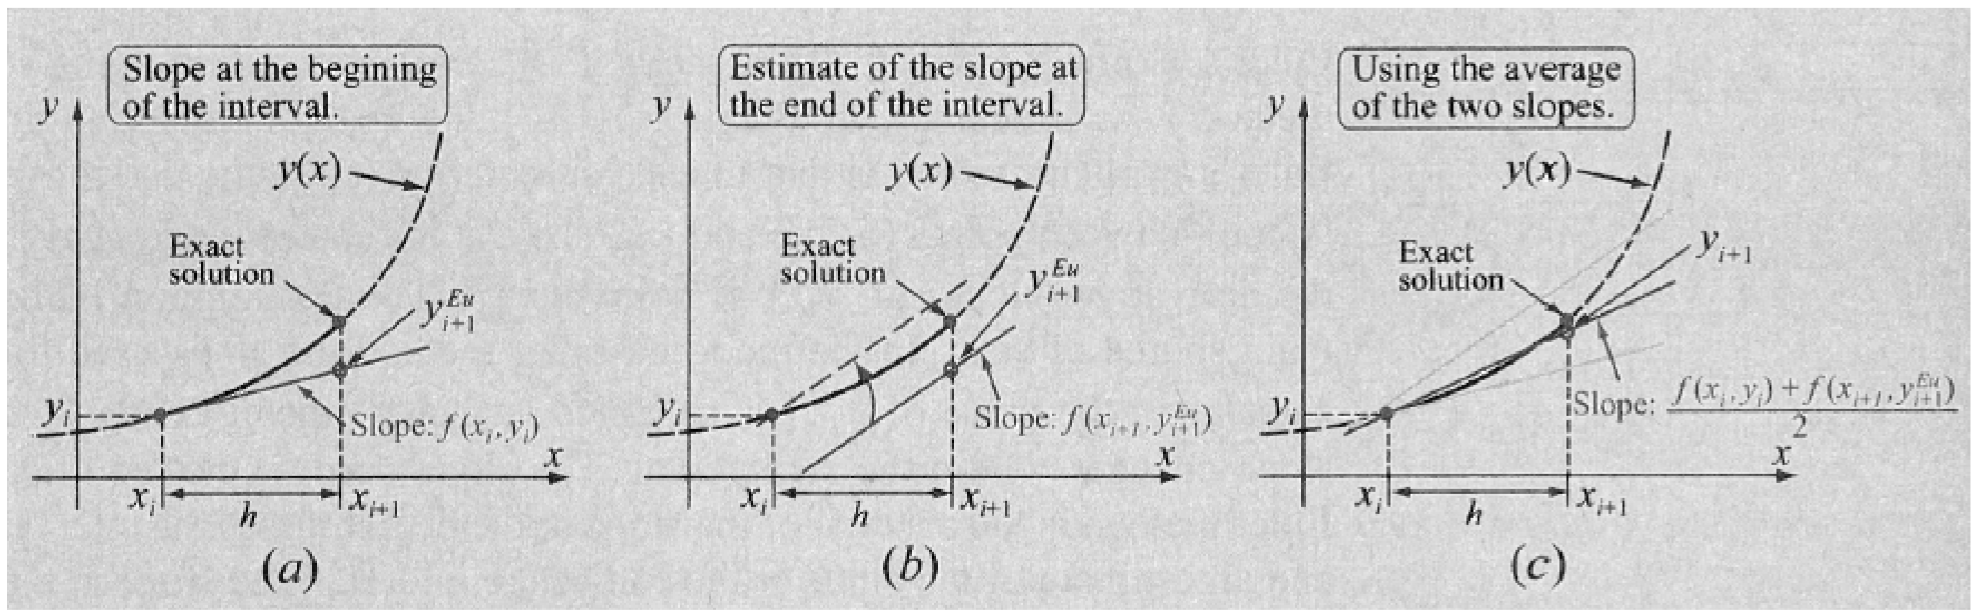
\includegraphics[width=500px]{img/EulerischeVerfahrenImUeberblick.png}
	\captionof{figure}{Überblick der eulerischen Verfahren}
	\label{fig:Überblick der eulerischen Verfahren}
\end{Figure}

\textbf{Beispiel modifiziertes Euler-Verfahren}\\
\textit{Wie berechnen die numerische Lösung des Anfangsproblems $y'(t) = t(t,y(t)) = ^2 + 0.1 * y(t)$ mit y(-1.5)=0 auf dem Intervall $[a,b] = [-1.5,1.5]$ und n = 5, mit dem modifizierten Euler-Verfahren}
\begin{equation}
\begin{split}
n &= 5 \Rightarrow h = \frac{b-a}{n} = \frac{1.5 - (-1.5)}{5} = 0.6\\
t_i &= a+ih = -1.5 + i * 0.6 \;(i = 0, 1,..., 5)\\
y_{i+1} &= y_i + h * \frac{(k_1 + k_2)}{2}
\end{split}
\end{equation}

\begin{Figure}
\centering
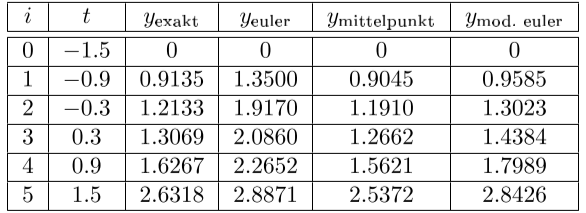
\includegraphics[width=200px]{img/VerfahrenVergleich.png}
	\captionof{figure}{Vergleich der kennengelernten Verfahren}
	\label{fig:Vergleich der kennengelernten Verfahren}
\end{Figure}
\begin{Figure}
\centering
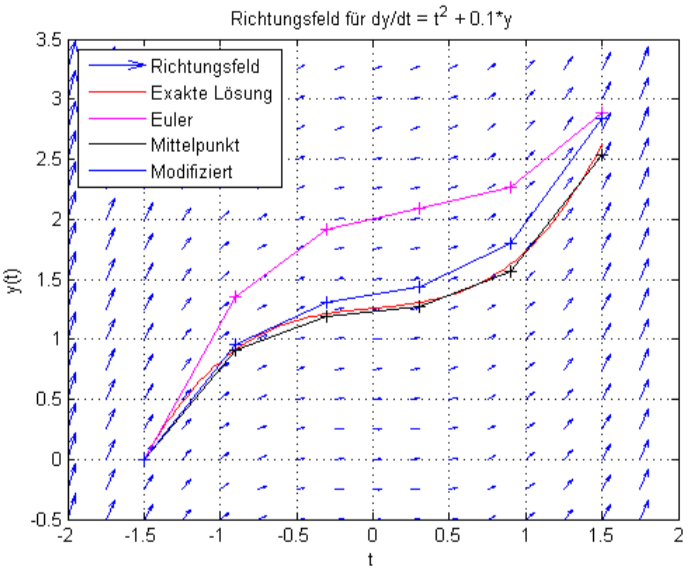
\includegraphics[width=200px]{img/VerfahrenVergleichRichtungsfeld.png}
	\captionof{figure}{Vergleich der kennengelernten Verfahren anhand des Richtungsfeldes}
	\label{fig:Vergleich der kennengelernten Verfahren anhand des Richtungsfeldes}
\end{Figure}

\subsection{Die Fehlerordnung eines Verfahrens}
Wie in der obigen Abbildung ersichtlich, kann sich der numerische Wert stark von der exakten Lösung unterscheiden. Damit wir dies genauer untersuchen können, führen wir die Begriffe \textit{lokalen Fehler} und \textit{globalen Fehler} sowie die jeweilige \textit{Fehlerordnung} ein.

\begin{tcolorbox}
\begin{definition}[\textbf{lokaler Fehler / Konistenzordnung}]
Sei $y'(x) = f(x,y(x))$ eine Differentialgleichung mit der Anfangsbedingung $y(x_i) = y_i$ und der exakten Lösung $y(x)$.\\
Sei $y_{i+1}$ der mit einem numerischen Näherungsverfahren mit der Schrittweite $h$ berechnete Näherungswert $y(x_{i+1})$, wobei $x_{i+1} = x_i + h$. Dann ist der \textbf{lokale Fehler} (also nach einer Iteration) definiert als die Differenz zwischen dem exakten Wert und der Näherung:
\begin{equation}
\varphi(x_i,h) := y(x_{i+1} - y_{i+1})
\end{equation}
Ein numerisches Verfahren hat die \textbf{Konsistenzordnung p} falls gilt:
\begin{equation}
|\varphi(x,h)|\leq C * h^{p+1} 
\end{equation}
für genügend kleine $h$ und einer Konstante $C > 0$, die von der Differentialgleichung abhängt.\\
\begin{Figure}
\centering
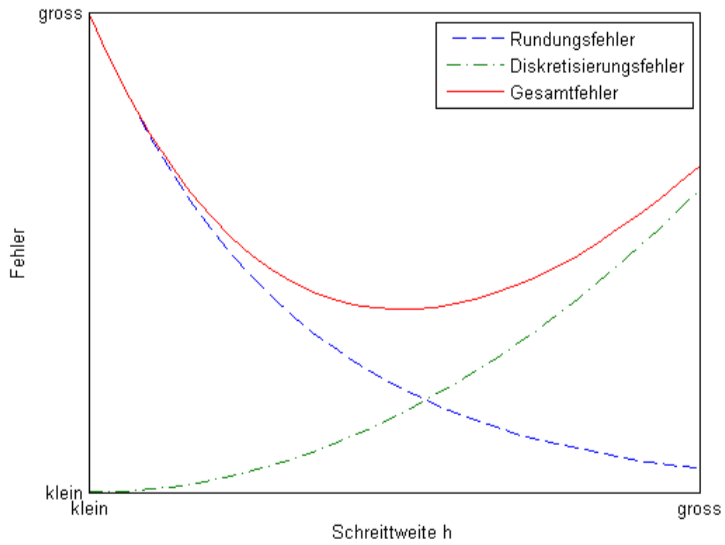
\includegraphics[width=200px]{img/lokalerFehler.png}
	\captionof{figure}{Verhalten des Rundungsfehlers und des Diskretisierungsfehlers}
	\label{fig:Verhalten des Rundungsfehlers und des Diskretisierungsfehlers}
\end{Figure}
\end{definition}
\end{tcolorbox}

\begin{tcolorbox}
\begin{definition}[\textbf{globaler Fehler / Konvergenzordnung}]
Sei $y'(x) = f(x, y(x))$ eine Differentialgleichung mit der Anfangsbedingung $y(x_0) = y_0$ und der exakten Lösung $y(x)$.
Sei $y_n$ der mit einem numerischen Näherungsverfahren mit der Schrittweite $h$ berechnete Näherungswert für $y(x_n)$, wobei $x_n = x_0 + nh$. Dann ist der Gesamtfehler (also nach \textit{n} Iterationen) bzw. der \textbf{globale Fehler} definiert als die Differenz zwischen dem exakten Wert und der Näherung:
\begin{equation}
y(x_n) - y_n
\end{equation}
Ein numerisches Verfahren hat die \textbf{Konvergenzordnung p} falls gilt:
\begin{equation}
|y(x_n) - y_n|\leq C * h^P
\end{equation}
für genügend kleine h und einer Konstante $C > 0$, die von der Differenzialgleichung abhängt.
\end{definition}
\end{tcolorbox}
\textit{Bemerkungen}\\
\begin{itemize}
\item Der lokale Fehler ist ein Mass für die Abweichung von der exakten Lösung nach einer Iteratino, während der globale Fehler die Abweichung von der exakten Lösung nach \textit{n} Iterationen misst.
\item Die hier gemachten Definitionen beziehen sich nur auf den Diskretisierungsfehler. Es kommt noch der Rundungsfehler hinzu. 
\item Für die hier betrachteten Verfahren ist die Konsistenz- und Konvergenzordnung jeweils identisch
\item {Verwendbar sind nur Verfahren mit der Konvergenzordnung $p \leq 1$, da dann der globale Fehler gegen Null strebt:
\begin{equation}
\lim_{h \rightarrow 0} |y(x_n) - y_n| \leq \lim_{h \rightarrow 0} C * h^P = 0
\end{equation}
}
\end{itemize}
Das bedeutet, der Diskretisierungsfehler wird theoretisch beliebig klein, wenn die Schrittweite $h$ beliebig klein wird. In der Praxis verhindern natürlich Rundungsfehler, dass eine beliebige Genauigkeit erzielt werden kann.

\subsection{Runge-Kutta Verfahren}
Im Einzelschrittverfahren wird die Steigung im Richtungsfeld verwendet gemäss:
\begin{equation}
\begin{split}
x_{i+1} &= x_i + h\\
y_{i+1} &= y_i + \textit{Steigung} * h
\end{split}
\end{equation}
Das klassische Euler-Verfahren verwendet einen Punkt, um die Steigung zu berechnen und hat die Konsistenz- und Konvergenzordnung $p=1$. Das Mittelpunkt-Verfahren und das modifizierte Euler-Verfahren verwenden dazu zwei Punkte und haben die Konsistenz- und Konvergenzordnung $p=2$.\\
Offenbar kann durch die Hinzunahme von zusätzlichen Punkten zur Berechnung eines Durchschnitt-Werts für die Steigung die Genauigkeit eines Einschrittverfahrens verbessert werden.

\subsubsection{Das klassische vierstufige Runge-Kutta Verfahren}
\begin{tcolorbox}
\begin{definition}[\textbf{Algorithmus: klassisches vierstufige Runge-Kutta Verfahren}]
Gegeben sei für $x \in [a,b]$ das Anfangswertproblem
\begin{equation}
y' = f(x,y) \textrm{ mit } y(a) = y_0
\end{equation}
Das klassische Runge-Kutta zur numerischen Lösung lautet
\begin{equation}
\begin{split}
k_1 &= f(x_i, y_i)\\
k_2 &= f(x_i + \frac{h}{2}, y_i + \frac{h}{2}k_1)\\
k_3 &= f(x_i + \frac{h}{2}, y_i + \frac{h}{2}k_2)\\
k_4 &= f(x_i + h, y_i + h k_3)\\
x_{i+1} &= x_i + h\\
y_{i+1} &= y_i + h*\frac{1}{6}(k_1 + 2k_2 + 2k_3 + k_4) 
\end{split}
\end{equation}
wobei $x_0 = a, x_i = a + ih$ für i = 0,..., n-1 ($n \in \mathbb{N}$) und $h = \frac{b-a}{n}$
\end{definition}
\end{tcolorbox}
\begin{Figure}
\centering
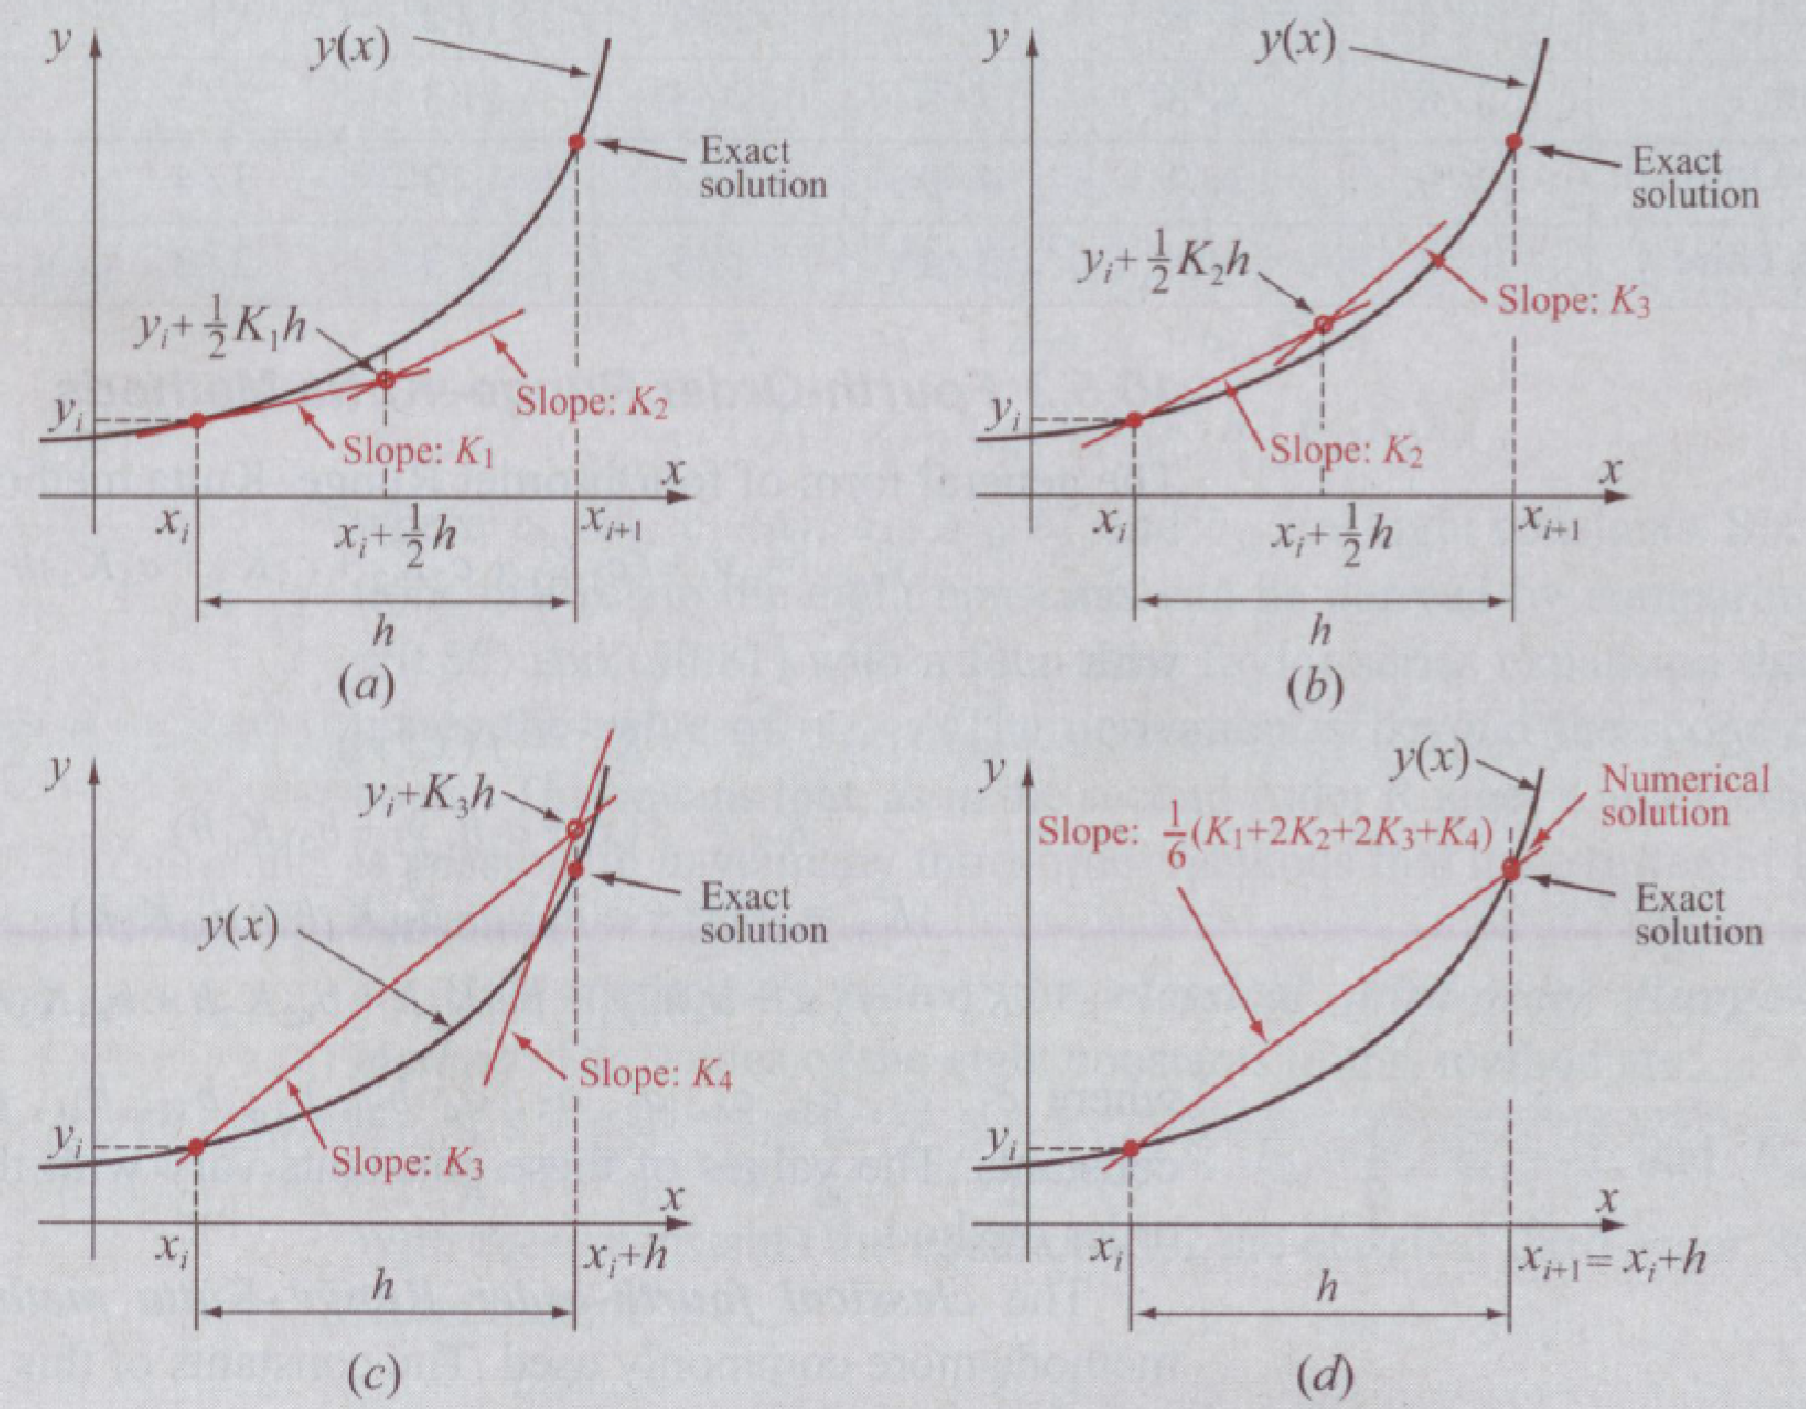
\includegraphics[width=200px]{img/vierfachesRungeKuttaVerfahren.png}
	\captionof{figure}{Klassisches vierstufiges Runge-Kutta-Verfahren}
	\label{fig:Klassisches vierstufiges Runge-Kutta-Verfahren}
\end{Figure}
\textit{Das klassische vierstufige Runge-Kutta Verfahren hat die Konsistenz- und Konvergenzordnung p = 4}\\

\textbf{Beispiel Runge-Kutta Verfahren}\\
\textit{Wir berechnen wieder die numerische Lösung des Anfangswertproblems}
\begin{equation}
y'(t) = f(t,y(t)) = t^2 + 0.1 * y(t)
\end{equation}
mit y(-1.5) = 0 auf dem Intervall $[a,b] = [-1.5, 1.5]$ und n = 5, diesmal aber mit klassischen Runge-Kutta Verfahren.\\
\textit{Klassisches Runge-Kutta Verfahren}
\begin{Figure}
\centering
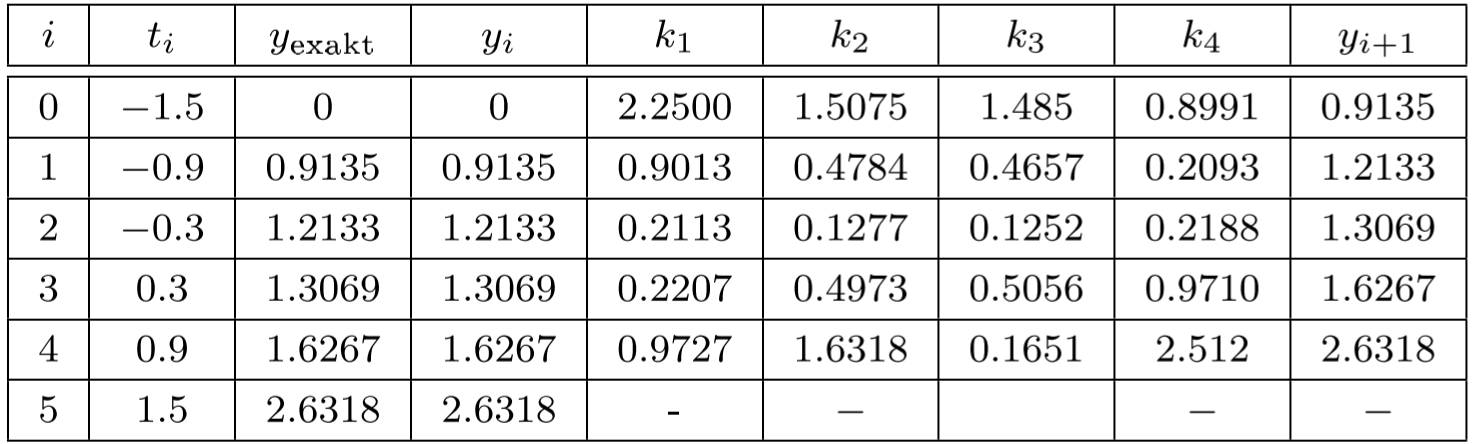
\includegraphics[width=200px]{img/RungeKuttaVerfahren.png}
	\captionof{figure}{Klassisches Runge-Kutta-Verfahren}
	\label{fig:Klassisches Runge-Kutta-Verfahren}
\end{Figure}
Der Vergleich mit den Werten der exakten Lösung $y_{exakt}$ bei dieser Genauigkeit keinen Unterschied mehr\\
\begin{Figure}
\centering
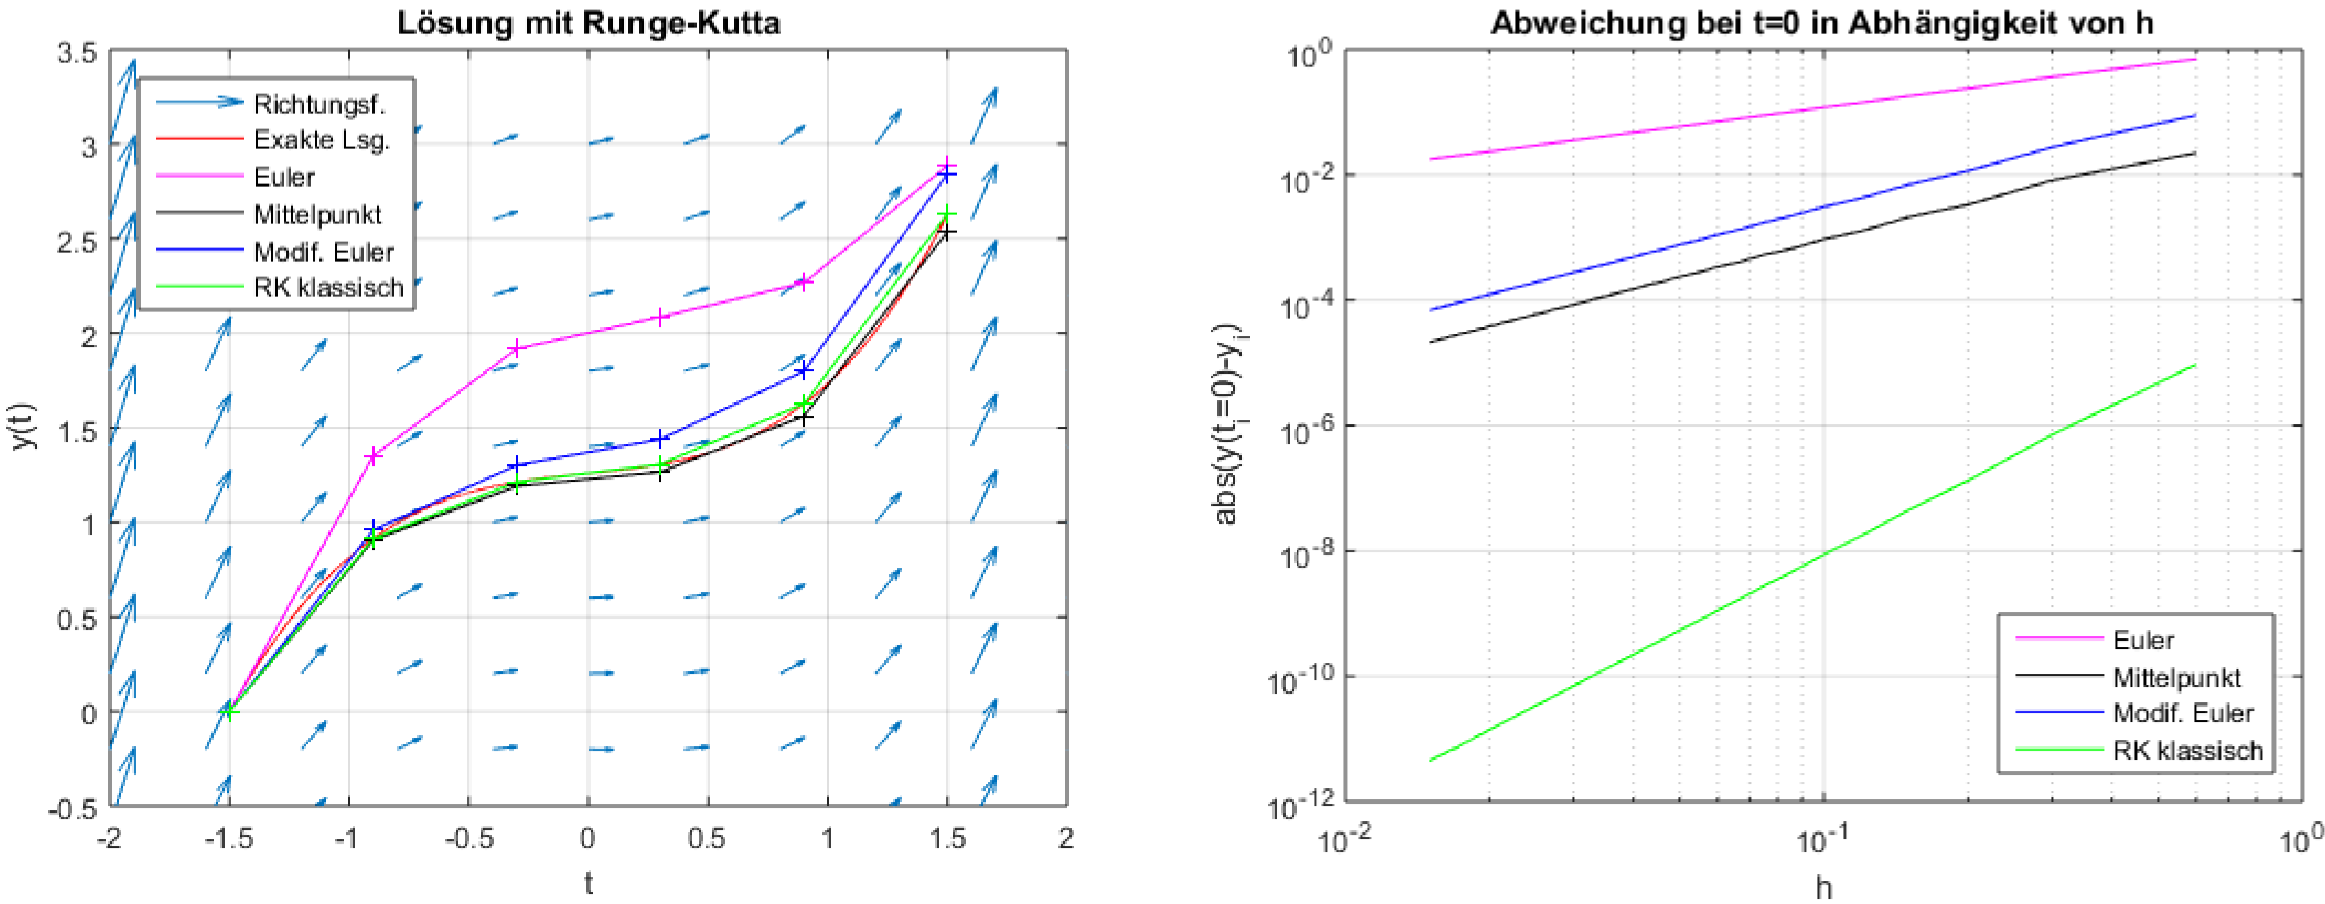
\includegraphics[width=400px]{img/verschiedeneVerfahrenInklRungeKutta.png}
	\captionof{figure}{Vergleich von verschiedenen Verfahren inkl. Runge-Kutta (links)}
	\label{fig:Klassisches Runge-Kutta-Verfahren}
\end{Figure}

\subsubsection{Das allgemeine s-stufige Runge-Kutta Verfahren}
\begin{tcolorbox}
\begin{definition}[\textbf{Allgemeines s-stufiges Runge-Kutta Verfahren}]
Ein allgemeines (explizites) s-stufiges Runge-Kutta Verfahren ist gegeben durch die Formeln
\begin{equation}
\begin{split}
k_n &= f(x_i + c_n h, y_i + h \sum\limits_{m=1}^{n-1} a_{nm}k_{m}) \textrm{ für n = 1,... ,s}\\
y_{i+1} &= y_i + h \sum\limits_{n=1}^{s} b_n k_n 
\end{split}
\end{equation}
Hierbei ist $s \in \mathbb{N}$ die Stufenzahl und $a_{bm}, b_n, c_n$ sind Konstanten. Die Konstistenz- und Konvergenzordnung hängt von der Wahl dieser Konstanten ab
\end{definition}
\end{tcolorbox}
\textit{Bemerkung: } Man notiert die Koeffizienten meist in der Form
\begin{Figure}
\centering
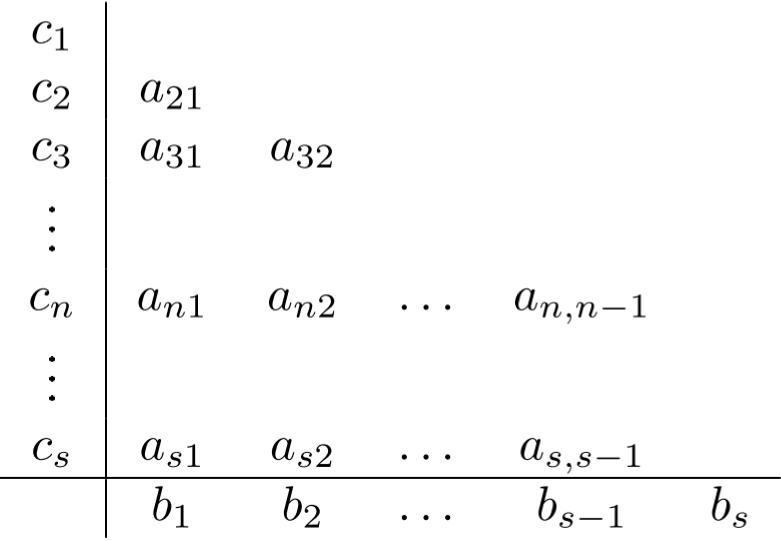
\includegraphics[width=200px]{img/KoeffizientenForm.png}
	\captionof{figure}{Koeffizienten Formen}
	\label{fig:Koeffizienten Formen}
\end{Figure}

\subsection{Mehrschrittverfahren}
Bei Mehrschrittverfahren im Gegensatz zu den Einschrittverfahren für die Berechnung von $y_{i+1}$ nicht nur der vorhergehende Punkt ($x_i$, $y_i$) benötigt, sondern mindestens zwei (also z.B. ($x_i$, $y_i$) und ($x_{i−1}$, $y_{i−1}$)) oder noch mehr vorhergehende Punkte.\\
Wir beschreiben hier die Familie der (expliziten) Adams Bashforth Methoden.\\
Die Lösung der DGL
\begin{equation}
y' = f(x,y)
\end{equation}
wird dabei durch Integration über das Intervall $[x_i, x_{i+1}]$ erreicht:
\begin{equation}
y_{i+1} = y_i + \int\limits_{x_i}^{x_{i+1}} f(x,y)dx
\end{equation}
Dabei wird f(x,y) durch ein Polynom angenähert, welches die Werte von f(x,y) bei ($x_i$,$y_i$) und vorhergehenden Punkten interpoliert. Je nach Ordnung des verwendeten Polynoms erhält man eine andere Iterationsvorschrift.

\subsubsection{Adams-Bashforth Methode 2. und 3. Ordnung}
Verwendet man die Punkte $(x_i, y_i)$ und $(x_{i-1}, y_{i-1})$, dann ist das interpolierende Polynom vom Grad 1 (eine Gerade) und es gilt:
\begin{equation}
f(x,y) = f(x_i, y_i) + \frac{f(x_i, y_i) - f(x_{i-1}, y_{i-1})}{h}*(x-x_1)
\end{equation}
mit $h = x_{i+1} - x_i$. Durch die Integration erhalten wir dann:
\begin{equation}
\begin{split}
y_{i+1} &= y_i + \int\limits_{x_i}^{x_{i+1}} f(x,y)dx\\
&= y_i + \int\limits_{x_i}^{x_{i+1}} f(x,y)dx + \int\limits_{x_i}^{x_{i+1}} \frac{f(x_i, y_i) - f(x_{i-1}, y_{i-1}}{h}*(x-x_i)dx\\
&= y_i + f(x_i, y_i) \int\limits_{x_i}^{x_{i+1}} dx + \frac{f(x_i, y_i) - f(x_{i-1}, y_{i-1}}{h} \int\limits_{x_i}^{x_{i+1}}(x-x_i)dx\\
&= y_i + f(x_i, y_i) * (x_{i+1}-x_i) + \frac{f(x_i, y_i) - f(x_{i-1}, y_{i-1})}{h}*\frac{1}{2}(x_{i+1} - x_i)^2\\
&= y_i + f(x_i, y_i) * h + (f(x_i, y_i) - f(x_{i-1}, y_{i-1})) * \frac{1}{2}h\\
&= y_i + \frac{h}{2}(3f(x_i, y_i) - f(x_{i-1}, y_{i-1}))
\end{split}
\end{equation}

Die Iteration
\begin{equation}
y_{i+1} = y_i + \frac{h}{2}(3f(x_i, y_i) - f(x_{i-1}, y_{i-1}))
\end{equation}
ist die Adams-Bashforth Methode 2. Ordnung. Denn diese verwendet zwei Punkte. Diese Methode kann erst ab dem zweiten Punkt $(x_2, y_2)$ verwendet werden, da die Punkte $(x_0, y_0)$ und $(x_1, y_1)$ für die Iteration bekannt sein müssen. Dementsprechend muss für die Berechnung von $(x_1, y_1)$  ein Einschrittverfahren verwendet werden. \\
Durch die Verwendung eines Polynoms vom Grad 3 (Parabel) kann $f(x,y)$ in den Punkten $(x_i, y_i)$, $(x_{i-1}, y_{i-1})$ und $(x_{i-2}, y_{i-2})$ interpoliert werden und wir erhalten die Adams-Bashforth Methode 3. Ordnung, welche ab $(x_3, y_3)$ einsetzbar ist:
\begin{equation}
y_{i+1} = y_i + \frac{h}{12}(23f(x_i, y_i) - 16 f(x_{i-1}, y_{i-1}) + 5f(x_{i-2}, y_{i-2}))
\end{equation}

\subsubsection{Adams Bashforth Methoden höherer Ordnung}
Durch die Verwendung eines Interpolationpolynoms vom Grad \textit{s} erhält man die Adams Bashforth Methode der Ordnung \textit{s+1} über die generelle Formel:
\begin{equation}
	y_{i+} = y_1 + \sum_{j=0}^{s} b_j f(x_{i-j}, y_{i-j})
\end{equation}
mit den Koeffizienten
\begin{equation}
	b_j = \frac{(-1)^j}{j!(s-j)!}\int_0^1 \prod_{k=0, k\neq j}^s (u+k)du \quad j=0,1,...,s
\end{equation}

\subsection{Erweiterung auf Systeme von Differentialgleichungen}
Die bisherigen System sind nur für Differentialgleichungen 1. Ordnung anwendbar. \\
Wir zeigen nun:
\begin{itemize}
	\item[i)] Wie aus einer Differentialgleichung k-ter Ordnung ein System von \textit{k} Differentialgleichungen 1. Ordnung gemacht
	\item[ii)] wie dieses System anschliessend mit den uns bereits bekannten Verfahren gelöst werden kann
\end{itemize}

\subsection{Zurückführe einer DGL \textit{k}-ter Ordnung auf \textit{k} DGL 1. Ordnung}
\textbf{evtl Beispiel 7.9 S.129 einfügen}\\

\begin{tcolorbox}
\begin{definition}[\textbf{Rezept für das Zurückführen auf ein System erster Ordnung}]
\begin{enumerate}
	\item Die Differentialgleichung nach den höchsten vorkommenden Ableitungen der unbekannten Funktion auflösen
	\item Neue Funktionen für die unbekannten Funktionen und deren Ableitung bis Ordnung der höchsten Ableitung minus 1 einführen
	\item Das System erster Ordnung durch Ersetzen der höheren Ableitungen durch die neue Funktionen aufstellen
	\item Das entsprechende Anfangswertproblem in vektorieller Form aufschreiben
\end{enumerate}
\end{definition}
\end{tcolorbox}

\subsection{Lösen eines Systems von \textit{k} DGL 1. Ordnung}
\textbf{evtl Beispiel 7.9 S.130 weiterführen}\\

\begin{tcolorbox}
\begin{definition}[\textbf{Rezept für das Lösen eines Systems von \textit{k} DGL 1. Ordnung}]
Ist ein Lösungs-Verfahren
\begin{equation}
\begin{split}
	x_{i+1} &= x_1 + h\\
	y_{i+1} &= y_i + Steigung * h
\end{split}
\end{equation}
für die eindimensionale Gleichung
\begin{equation}
x'(x) = f(x,y(x)), y(x_0) = y_0
\end{equation}
definiert, so kann es völlig analog erweitert werden als
\begin{equation}
\begin{split}
x_i &= x_i + h\\
\textbf{y}^{(i+1)} &= \textbf{y}^{(i+1)} + Steigung * h
\end{split}
\end{equation}
für ein System
\begin{equation}
\textbf{y'} = \textbf{f}(x,\textbf{y}(x)) \; \textrm{ mit } \textbf{y}(x_0) = \textbf{y}^{(0)}
\end{equation}
(wobei wie üblich ein hochgestellter Index in Klammern $y^{(i)}$ einen Vektor aus $\mathbb{R}^n$ nach der i-ten Iteration bezeichnet).\\
Dabei werden ersetzt:
\begin{itemize}
	\item y' durch den Vektor \textbf{y'} der Ableitungen der einzelnen Komponenten
	\item f(x,y(x)) durch die vektorwertige Funktion $\textbf{f}(x,\textbf{y}(x))$ und
	\item die skalare Anfangsbedingung $y(x_0) = y_0$ durch die Anfangsbedingung $\textbf{y}(x_0) = \textbf{y}^{(0)}$
\end{itemize}
Es ist dann also:
\begin{equation}
\textbf{y}(x) = \begin{pmatrix}
y_1(x)\\
y_2(x)\\
.\\
.\\
.\\
y_n(x)
\end{pmatrix}, \textbf{y}' = \begin{pmatrix}
y'_1(x)\\
y'_2(x)\\
.\\
.\\
.\\
y'_n(x)
\end{pmatrix}, \textbf{f}(x,\textbf{y}(x)) = \begin{pmatrix}
f_1(x,\textbf{y}(x))\\
f_2(x,\textbf{y}(x))\\
.\\
.\\
.\\
f_n(x,\textbf{y}(x))\\
\end{pmatrix}, \textbf{y}(x_0) = \textbf{y}^{(0)} = \begin{pmatrix}
y_1(x_0)\\
y_2(x_0)\\
.\\
.\\
.\\
y_n(x_0)
\end{pmatrix}
\end{equation}
\textbf{Bemerkung:} Wurd das System erstellt, um eine DGL k-ter Ordnung zu lösen, so finden sich die Lösung $y(x)$ in der ersten Komponente des Vektors \textbf{y}(x), als $y(x) \approx y_1(x)$
\end{definition}
\end{tcolorbox}

\subsection{Stabilität}
Der Fehler bei der Lösung einer DGL setzt sich aus dem vom benutzten Verfahren abhängigen Diskretisierungsfehler und dem vom Rechner abhängigen Rundungsfehler zusammen. In gewissen Situation kann der numerische Fehler im Verlauf der Iteration unbeschränkt gross werden (unabhängig der Schrittweite h). Dabei spricht man von \textit{Instabilität} bzw. von einer instabilen Lösung. Die Stabilität einer Lösung hängt von drei Faktoren ab:
\begin{itemize}
	\item[i.)] dem benutzen Verfahren
	\item[ii.)] der Schrittweite h
	\item[iii.)] dem spezifischen Anfangswertproblem
\end{itemize}
Dabei gibt es verschiedene Methoden, um das Problem zu untersuchen, z.B.:
\begin{itemize}
	\item Durchrechnen der Lösung einmal mit single- und einmal mit double-precision mit anschliessendem Vergleich. $\rightarrow$ Dies kann Aussagen möglich machen zur Akkumulation von Rundungsfehlern
	\item Variation der Schrittweite \textit{h}. $\rightarrow$ dies erlaubt Aussagen zum Diskretisierungsfehler
	\item Vergleich der Resultate erzielt mit einem Lösungsverfahren höherer Ordnung und einem Lösungsverfahren niederer Ordnung
	\item Vergleich der Resultate eines numerischen Lösungsverfahrens mit der analytischen Lösungs, sofern diese bekannt ist.
\end{itemize}
Den letzten Punkt schauen wir genauer an:\\
Das Anfangsproblem
\begin{equation}
	y' = -\alpha y, y(0) = y_0 = 1 (\alpha > 0)
\end{equation}
für welches wir die exakte Lösung kennen:
\begin{equation}
y(x)= e^{-\alpha x}
\end{equation}
Das Euler-Verfahren liefert die numerische Lösung
\begin{equation}
	y_{i+1} = y_i - h * \alpha y_i = <_i(1-h \alpha)
\end{equation}
Durch rekursives Einsetzen von $y_i = y_{i-1} (1-h\alpha)$ erhalten wir:
\begin{equation}
y_{i+1} = y_i * (1-h\alpha) = y_{i-1} (1-h\alpha)^2 = y_{i-2}(1-h\alpha)^3 = ... = \underbrace{y_0}_{\substack{=1}}(1-h\alpha)^{i+1}
\end{equation}
Da die exakte Lösung $y = e^{-\alpha x}$ streng monoton fallend ist, sollte auch die Näherungslösung streng monoton fallend sein, d.h. in diesem Fall
\begin{equation}
|1 - h \alpha | < 1
\end{equation}
und es folgt
\begin{equation}
0 < h \alpha < 2 \Rightarrow 0 < h < \frac{2}{\alpha}
\end{equation}
Wir haben also eine obere Schranke für \textit{h} hergeleitet bzw. eine Schrittweitenobergrenze für die die numerische Lösung stabil bleibt. 

\begin{tcolorbox}
\begin{definition}[\textbf{Stabilitätsfunktion / Stabilitätsinterval}]
Kann bei der Anwendung eines Verfahrens auf die DGL $y' = -\alpha y$ die numerische Lösung in der Form
\begin{equation}
y_{i+1} = g(h \alpha) * y_i
\end{equation}
geschrieben werden, so nennt man $g(z)$ die Stabilitätsfunktion des Verfahrens ( mit $z = h \alpha$)\\
Das offene Intervall $z \in (0, \alpha)$, in dem $|g(z)|<1$ gilt, bezeichnet man als das Stabilitätsinterval des Verfahrens
\begin{Figure}
\centering
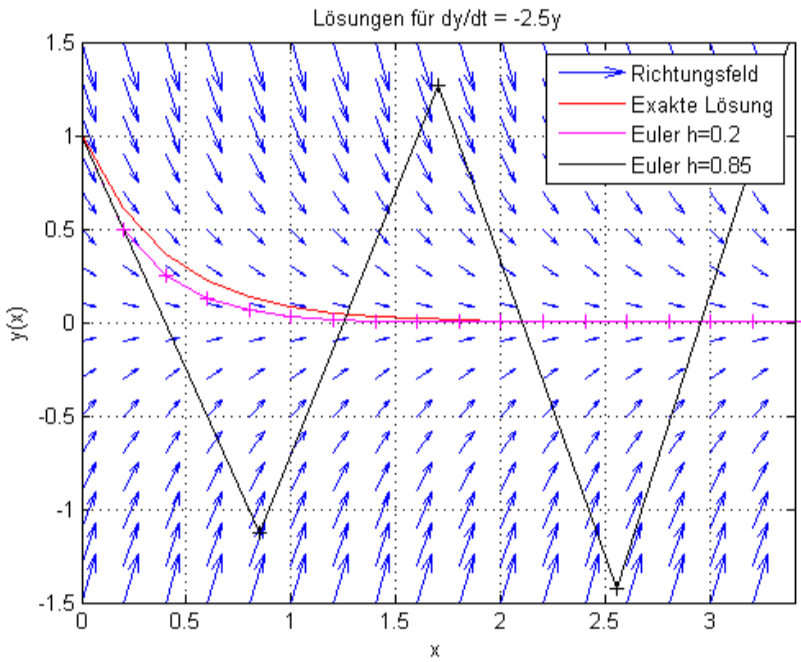
\includegraphics[width=200px]{img/RichtungsfeldEulerVerfahren.png}
	\captionof{figure}{Euler-Verfahren für die Lösung der DGL $y'=-2.5y$ mit den Schrittweiten $h_1 = 0.2$ (stabil) und $h_2 = 0.85$ (instabil)}
	\label{fig:Euler-Verfahren Stabilität}
\end{Figure}

\textbf{Bemerkungen:}\\
\begin{itemize}
\item Die Stabilitätsfunktion für das Euler-Verfahren ist $g(z) = 1 + z$
\item Man kann zeigen, dass die Stabilitätsfunktion eine s-stufigen (expliziten) Runge-Kutta Verfahrens ein Polynom vom Grad s ist.
\end{itemize}
\end{definition}
\end{tcolorbox}

\subsection{Weitere Punkte}
Zur Vollständigkeit werden weitere Punkte zur Differentialgleichungen betrachtet.

\subsubsection{Implizite vs. explizite Verfahren}
Bis anhin haben wir uns auf die Lösung von expliziten DGL der Form
\begin{equation}
y^{(n)}(x) = f(x, y(x), y'(x),...,y^{n-1}(x))
\end{equation}
beschränkt, d.h. die DGL ist nach der höchsten Ableitung aufgelöst. Wir haben demnach auch nur explizite Verfahren angewendet. Im Gegensatz dazu gibt es die impliziten DGL der Form:
\begin{equation}
F(x,y(x), y'(x),...,y^{(n-1)}(x), y^{(n)}(x)) = 0
\end{equation}
die nicht nach der höchsten Ableitung aufgelöst sind. Bei den zugehörigen impliziten Lösungsverfahren muss jeweils noch ein Nullstellenproblem gelöst werden (bspw. mit Newton-Verfahren), wie beim impliziten Euler-Verfahren
\begin{equation}
\begin{split}
x_{i+1} &= x_i + h\\
y_{i+} &= y_i+h*f(x_{i+1}, y_{i+1})
\end{split}
\end{equation}
da hier die gesuchte Lösung $y_{i+1}$ auf beiden Seiten der Gleichung auftaucht. Diese Verfahren sind deshalb aufwendiger, aber auch stabiler als die expliziten Verfahren. 

\subsubsection{Steife DGL}
Im Zusammenhang mit der Stabilitätsüberlegungen, redet man auch von sogenannten \textit{steifen DGL}. Diese sind DGL mit stark schwankenden Zeitskalen \textit{t} (oder Längeskalen x) der Lösung y. Zur Lösung solcher steifen DGL benötigen explizite Lösungsverfahren eine verschwindend kleine Schrittweite h, so dass die Lösung wegen langer Laufzeiten unpraktikabel oder wegen zunehmenden Rundungsfehler instabil wird. Steife DGL werden deshalb mit impliziten Verfahren gelöst.

\subsubsection{Schrittweitensteuerung}
Für DGL mit stark schwankenden Lösungsfunktionen $y(x)$ ist es effizienter, statt einer konstanten Schrittweite $h = \frac{b-a}{n} = const$ eine Variable Schrittweite h, anzuwenden, die klein ist in Bereichen grosser Krümmung der Lösung $y(x)$ und gross in Bereichen mit kleiner Krümmung. Hierzu sind Fehlerschätzungen für den lokalen Fehler nötig.

\subsubsection{MATLAB Funktionein zur Lösungs von Anfangswertproblemen}
\begin{itemize}
	\item {ode45 $\rightarrow$ Für nicht steife DGL. Einzelschritt-Verfahren basierend auf Runge-Kutta Verfahren der vierten und fünften Stufe. Gut als erster Versuch für viele Anfangswertprobleme.}
	\item {ode23 $\rightarrow$ Für nicht steife DGL. Einzelschritt-Verfahren basierend auf Runge-Kutta Verfahren der zweiten und dritten Stufe. Häufig schneller aber weniger genau als ode45}
	\item {ode113 $\rightarrow$ Für nicht steife DGL. Mehrschrittverfahren basierend auf Adams-Bashforth(-Moulton) Methoden.}
	\item {ode15s $\rightarrow$ Für steife DGL. Benutzt ein Mehrschritt-Verfahren. Tiefe bis mittlere Genauigkeit}
	\item {ode23s $\rightarrow$ Für steife DGL. Einzelschrittverfahren. Anwendbar auf einige Fälle die ode15s nicht lösen kann. Tiefe Genauigkeit}
	\item {ode23t $\rightarrow$ Für moderat steife DGL. Tiefe Genauigkeit}
	\item {ode23tb $\rightarrow$ Für steife DGL. Basiert auf einem impliziten Runge-Kutta Verfahren. Oft effizienter als ode15s.}
\end{itemize}

\section{Interpolation}

\subsection{Lernziele}
\begin{itemize}
	\item {Sie können mittels der Lagrange - Interpolationsformel und dem Aitken-Neville Schema eine Anzahl Messpunkte durch ein Polynom interpolieren und dieses Schema in MATLAB implementieren}
	\item Sie können für vorgegebene Stützpunkte die natürliche kubische Splinefunktion berechnen.
\end{itemize}

\subsection{Problemstellung}
Bei der Interpolation geht es darum bei einer Wertetabelle, die Lücken aufweist, die fehlenden Funktionswerte anzunähern. Es sei also eine Wertetabelle einer Funktion f mit $y_i = f(x_i)$ der Art
\begin{Figure}
\centering
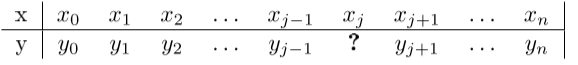
\includegraphics[width=200px]{img/WertetabelleInterpolation.png}
	\captionof{figure}{Allgemeine Wertetabelle Interpolation}
	\label{fig:Allgemeine Wertetabelle Interpolation}
\end{Figure}
gegeben. Die Wertepaare $(x_i, y_i)$ heissen \textbf{Stützpunkte}, die $x_i$ \textbf{Stützstelle} und die $y_i$ \textbf{Stützwerte}. Gesucht ist nun eine möglichstgute Näherung des fehlenden Wertes $y_i$. Dementsprechend sind wir auf der Suche nach einer (stetigen) Funktion, welche die eigentliche Funktion $f(x)$ an der Stelle $f(x_j)$ möglichst gut annähert und exakt durch die bekannten Stützpunkte in der Umgebung $x_j$ geht. Eine solche Funktion nennt man \textbf{Interpolierende}. Interpolatino kommt vor allen zur Anwendung, wenn die Funktion $f(x)$ nicht genügend bekannt oder nur schwer exakt zu berechnen ist. (Bspw. die digitale Bildbearbeitung)

\theoremstyle{definition}
\begin{tcolorbox}
\begin{definition}[Interpolationsproblem]
Gegeben sind $n+1$ Wertepaare $(x_i, y_i)$, i = 0, ..., n mit $x_i \neq x_j$ für  $i \neq j$ Gesucht ist eine stetige Funktion g mit der Eigenschaft $g(x_i) = y_i$ für alle i = 0, ..., n 
\end{definition}
\end{tcolorbox}

\subsection{Polynominterpolation}
Gegeben sind $n+1$ Stützpunkte
\begin{Figure}
\centering
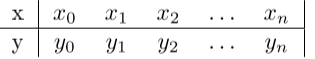
\includegraphics[width=200px]{img/Stuetzpunkte.png}
	\captionof{figure}{gegebene Stützpunkte}
	\label{fig:gegebene Stützpunkte}
\end{Figure}
und gesucht ist ein Polynom $P_n(x)$, welches diese Punkte interpoliert. Wenn wir uns das Polynom in der üblichen Form nach Potenzen von x entwickelt denken, dann ist
\begin{equation}
	P_n(x) = a_0 + a_ix  + a_2x^2 + ... + a_nx^n
\end{equation} 
$\Rightarrow$ Jeder Stützpunkt gibt eine lineare Gleichung für die Bestimmung des Koeffizienten $a_k$. $\rightarrow$ wir erhalten gleich viele Gleichungen wie unbekannte Koeffizienten:
\begin{equation}
\begin{split}
	a_0 + a_1x_0 + a_2x_0^2 + ... + a_nx_0^n &= y_0\\
	a_0 + a_1x_1 + a_2x_1^2 + ... + a_nx_1^n &= y_1\\
	... =& ...\\
	a_0 + a_1x_n + a_2x_n^2 + ... + a_nx_n^n &= y_n
\end{split}
\end{equation}

\begin{Figure}
\centering
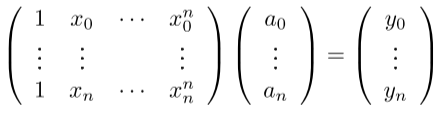
\includegraphics[width=200px]{img/InterpolationMatrix.png}
	\captionof{figure}{Vandermonde-Matrix}
	\label{fig:Vandermonde-Matrix}
\end{Figure}
Die Matrix wird Vandermonde-Matrix genannt. Im Prinzip könnten wir nun das lineare Gleichungssystem auflösen. Dies ist jedoch nicht effizient, da die Matrix typischerweise schlecht konditioniert ist. Durch eine andere Darstellung, lässt sich dies durchaus einfacher berechnen.

\theoremstyle{satz}
\begin{tcolorbox}
\begin{satz}[Lagrange Interpolationsformel]
Durch n+1 Stützpunkte mit verschiedenen Stützstellen (d.h. $x_i \neq x_j$, für $i \neq j$) gibt es genau ein Polynom $P_n(x)$ vom Grade $\geq$ n, welches alle Stützpunkte interpoliert, d.h. wo gilt
\begin{equation}
P_n(x_i) = y_i, i = 0,1,...,n
\end{equation}
$P_n(x)$ lautet in der Lagrangefrom
\begin{equation}
	P_n(x) = \sum\limits_{i=0}^n l_i(x) y_i
\end{equation} 
dabei sind die $l_i(x)$ die Lagrangepolynomae vom Grad n definiert durch
\begin{equation}
	l_i(x) = \prod\limits_{j=0, j\neq i} \frac{x-x_j}{x_i - x_j} \quad (i = 0, 1, ..., n)
\end{equation}
\end{satz}
\end{tcolorbox}
Für viele Aufgabenstellungen ist es einfacher, nicht ein Interpolationspolynom für alle gegebenen Stützpunkte zu berechnen, sondern nur die Punkte in unmittelbarer Umgebung des gesuchten Wertes zu berücksichtigen. Im einfachsten Fall nimmt man jeweils die zwei benachbarten Stützpunkte und verbindet sie mit einer Geraden. Das Interpolationspolynom ist dann also erster Ordnung und man spricht deshalb auch von \textit{(stückweise) linearer Interpolation}. Dazu gibt es wiederum eine Fehlerabschätzung:

\theoremstyle{satz}
\begin{tcolorbox}
\begin{satz}[Fehlerabschätzung]
Sind die $y_i$ Funktionswerte einer genügend oft stetig differenzierbaren Funktion $f$ als $y_i = f(x_i)$), dann ist der Interpolationsfehler an einer Stelle $x$ gegeben durch:
\begin{equation}
|f(x) - P_n(x)| \leq \frac{|(x-x_0)(x-x_1)...(x-x_n)|}{(n+1)!} max_{x_0 \leq \zeta \leq x_n}| f^{(n+1)}(\zeta)|
\end{equation}
\textbf{Bemerkung:} Wir müssen das Maximum der (n+1)-ten Ableitung der Funktion f(x) auf dem Intervall $[x_0,x_n]$ kennen. Entspricht ist die Fehlerabschätzung nur dann anwendbar, wenn wir die Funktion $f(x)$ und ihre Ableitung kennen.
\end{satz}
\end{tcolorbox}

Um die Lagrange-Polynome zu berechnen kann sehr aufwendig sein, aus diesem Grund führen wir nun eine Rekursionsformel ein. Diese macht die Berechnung der Interpolationspolynome $P_n(x)$ effizienter $\rightarrow$ \textit{Aitken-Neville Schema}. Es bezeichne dafür $p_{ij}(x)$ das Interpolationspolynom vom Grad $\leq j$ durch die Stützpunkte
\begin{Figure}
\centering
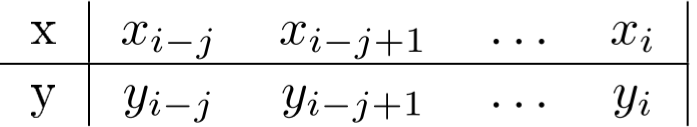
\includegraphics[width=200px]{img/AitkenNevilleStuetzpunkte.png}
	\captionof{figure}{Stützpunkte für das Aitken-Neville-Schema}
	\label{fig:Stützpunkte für das Aitken-Neville-Schema}
\end{Figure}

\theoremstyle{satz}
\begin{tcolorbox}
\begin{satz}[Aitken-Neville Schema]
Die Polynome $p_{ij}(x)$ lassen sich folgendermassen rekursiv berechnen: für i = 1,2,3,... und j = 1,2,...,i gilt
\begin{equation}
\begin{split}
p_{i0} &= y_i\\
p_{ij} &= \frac{(x_i-x)p_{i-1,j-1}+(x-x_{i-j}) p_{i,j-1}}{x_i-x_{i-j}}
\end{split}
\end{equation}
\begin{Figure}
\centering
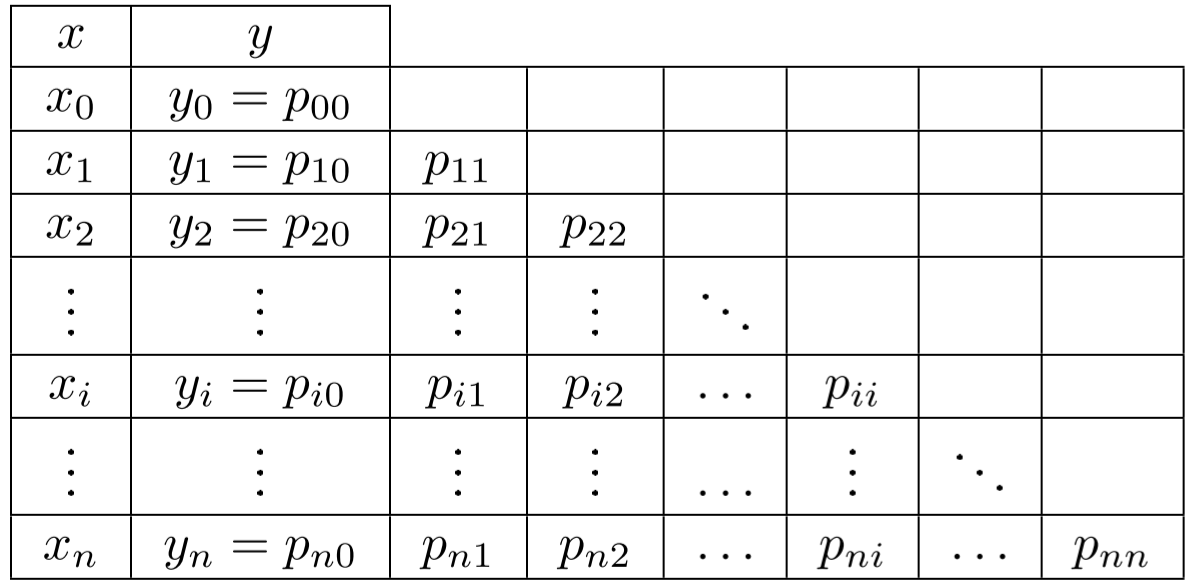
\includegraphics[width=200px]{img/AitkenNevilleSchema.png}
	\captionof{figure}{Schematische Darstellung für das Aitken-Neville-Schema}
	\label{fig:Schematische Darstellung für das Aitken-Neville-Schema}
\end{Figure}
Dabei müssen die $x_i$ in der ersten Spalte nicht unbedingt der Grösse nach sortiert sein. Ein Polynom $p_{ij}$ entspricht also dem Interpolationspolynom, welches die Punkte $x_0, x_1, ..., x_i$ interpoliert, aus diesem Grund gilt: $P_i(x) = p_{ij}(x)$ bzw. $P_n(x) = p_{nn}(x)$
\end{satz}
\end{tcolorbox}

\subsection{Splineinterpolation}
Polynome mit einem hohen Grad oszillieren (= schwingen). Dies führt dazu, dass bei einer grossen Anzahl Stützpunkten das Interpolationspolynom meist keine gute Näherung mehr für die zu interpolierende Funktion $f(x)$ darstellt.\\
Die Idee der Spline-Interpolation besteht nun darin, durch Polynome niederen Grades zu interpolieren und damit die Schwingungen zu unterdrücken, wobei man gleichzeitig sicherstellt, dass keine Knicke entstehen. Um diese zu erreichen, müssen die Polynome an den Anschlussstellen nicht nur denselber Funktionswert, sondern auch \textbf{dieselbe Ableitung} haben $\rightarrow$ Die Steigung der Tangente in diesen Punkten stimmt überein.

Wir wollen jetzt als Beispiel einen Algorithmus zur Berechnung der Koeffizienten für die natürliche kubische Splinefunktion kennen lernen:

\theoremstyle{definition}
\begin{tcolorbox}
\begin{definition}[\textbf{Algorithmus: natürliche kubische Splinefunktion}]
Gegeben seien $n+1$ Stützpunkte ($x_i,y_i$) mit monoton aufsteigenden Stützstellen (Knoten) $x_0 < x_1 < ... < x_n$ ($n\geq 2$).\\
Gesucht ist die natürliche kubische Splinefunktion S(x), welche in jedem Intervall $[x_i, x_i+1]$ mit i = 0, 1, ..., n-1 durch ein kubisches Polynom
\begin{equation}
S_i(x) = a_i + b_i(x-x_i)+c_i(x-x_i)^2+d_i(x-x_i)^3
\end{equation}
dargestellt wird als $S(x) = S_i(x)$ mit $x \in [x_i, x_{i+1}]$\\
Die Koeffizienten $a_i, b_i, c_i, d_i$ der Polynome $S_i(x)$ für i = 0, 1, ..., n-1 berechnen sich wie folgt:
\begin{enumerate}
	\item $a_i = y_1$
	\item $h_i = x_{i+1} - x_i$
	\item $c_0 = 0$, $c_n = 0$
	\item {Berechnung der Koeffizienten $c_1, c_2, ..., c_{n-1}$ aus dem Gleichungssystem
	\begin{itemize}
		\item[(a)] { $i=1$:\\
		$2(h_0 + h_1) c_1 + h_1c_2 = 3 \frac{y_2-y_1}{h_1} - 3\frac{y_1-y_0}{h_0}$}
		\item[(b)] {falls $n \geq 4$ gilt für i = 2, ..., n-2:\\
		$h_{i-1}c_{i-1}+2(h_{i-1}+h_i)c_i+h_ic_{i+1} = 3 \frac{y_{i+1} - y_i}{h_i}- 3 \frac{y_i - y_{i-1}}{h_{i-1}}$}
		\item[(c)] {$i = n-1$:\\
		$h_{n-2}c_{n-2} + 2(h_{n-2}+h_{n-1})c_{n-1} = 3\frac{y_n-y_{n-1}}{h_{n-1}} - 3 \frac{y_{n-1} - y_{n-2}}{h_{n-2}}$
		}
	\end{itemize}
	}	
	\item $b_i = \frac{y_{i+1} - y_i}{h_i} - \frac{h_i}{3} (c_{i+1} + 2c_i)$
	\item $d_i = \frac{1}{3h_i}(c_{i+1} - c_i)$
\end{enumerate}
Das Gleichungssystem unter Punkt 4 im Algorithmus hat die Form: $\textbf{Ac} = z$ mit:
\begin{Figure}
\centering
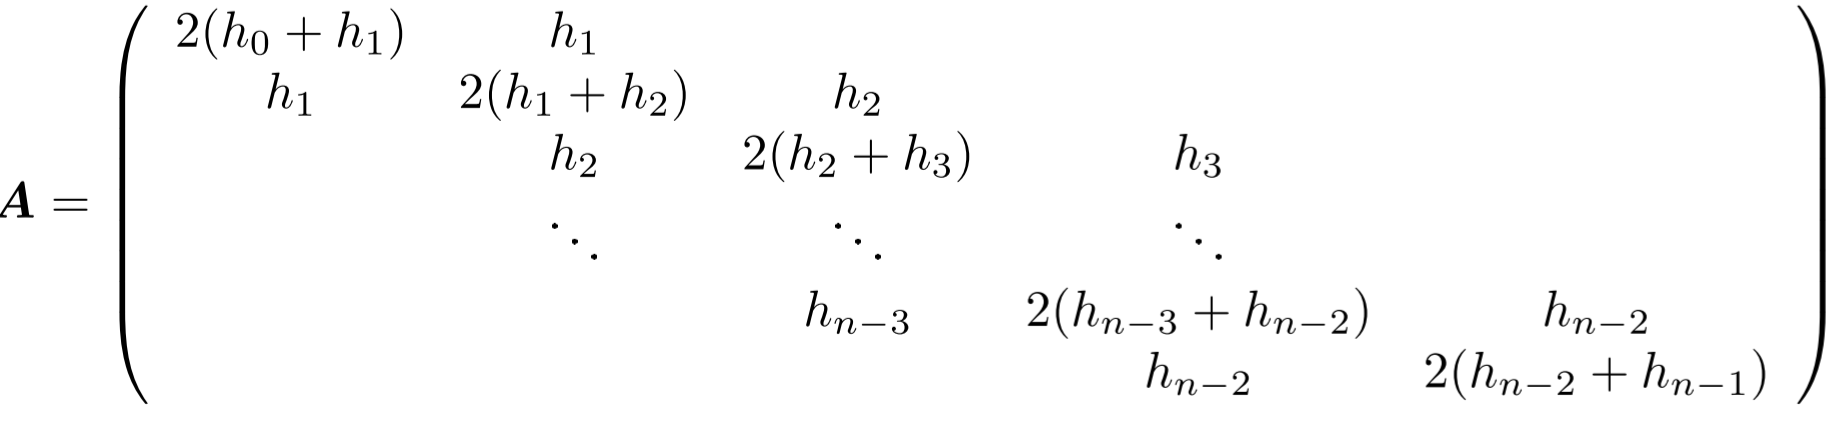
\includegraphics[width=200px]{img/kubischeSpineFunktionAForm.png}
	\captionof{figure}{A-Form für Algorithmus}
	\label{fig:A-Form für Algorithmus}
\end{Figure}
und
\begin{Figure}
\centering
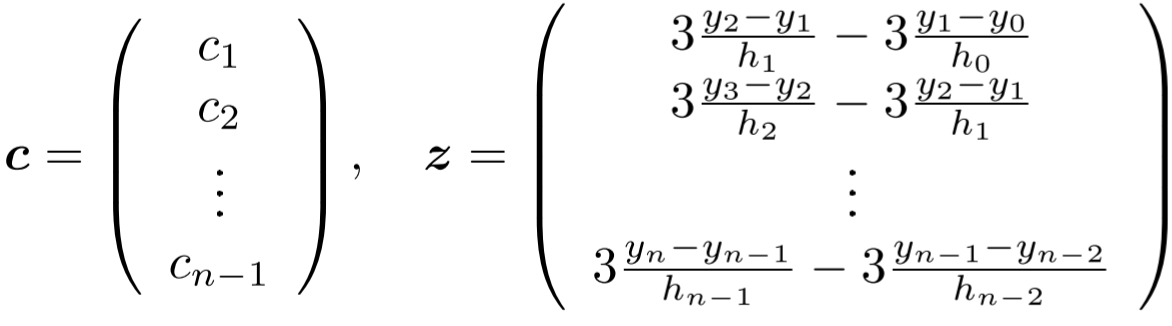
\includegraphics[width=200px]{img/kubischeSpineFunktionCForm.png}
	\captionof{figure}{c-Form für Algorithmus}
	\label{fig:c-Form für Algorithmus}
\end{Figure}
\textbf{Bemerkung: } Die Matrix A ist immer invertierbar. Zur numerischen Lösung sollte man den Gausschen-Algorithmus bzw. den Cholesky-Algorithmus verwenden. Das System ist gut konditioniert, Pivotsuche ist nicht erforderlich. Natürlich bietet MATLAB bereits fertige Funktionen bzw. eine ganze Toolbox für Splineinterpolation
\end{definition}
\end{tcolorbox}

\section{Ausgleichsrechnung}
Bei der Auswertung von Daten, will man häufig Datenpunkte mit einer gewissen Streuung durch eine relativ einfache Funktion annähern. Dabei sucht man eine Funktion, die möglichst nahe bei den Datenpunkte durchläuft, ohne dies exakt zu interpolieren. 
\subsection{Lernziele}
\begin{itemize}
	\item Sie können die Begriffe Ausgleichsproblem, Ansatzfunktion, Ausgleichsfunktion und Fehlerfunktional definieren
	\item Sie kennen die Optimierung des Fehlerfunktionals im Sinne der kleinsten Fehlerquadrate (least squares)
	\item Sie können das lineare sowie das allgemeine Ausgliechproblem definieren und für spezifische Beispiele lösen
	\item Sie können das gedämpfte Gauss-Newton Verfahren anwenden und in Matlab implementieren
\end{itemize}

\subsection{Problemstellung}
Im Unterschied zur Interpolation versuchen wir bei der Ausgleichsrechnung nicht, eine Funktion $f$ zu finden, die exakt durch sämtliche Wertepare geht, sondern diese nur möglichst gut approximiert. Dies ist insbesondere dann sinnvoll, wenn es eine grosse Anzahl von Datenpunkte gibt (die meist zusätzlich noch fehlerbehaftet sind) und die durch eine Funktion mit nur wenigen Paramtern beschrieben werden sollen.

\theoremstyle{definition}
\begin{tcolorbox}
\begin{definition}[\textbf{Ausgleichsproblem}]
Gegeben sind $n$ Wertpaare ($x_i, y_i$), i = 1, ..., n mit $x_i \neq x_j$ für $i \neq j$ \\
Gesucht ist eine stetige Funktion $f: \mathbb{R} \rightarrow \mathbb{R}$, die die Wertpaare in einem gewissen Sinn bestmöglich annähert, d.h. dass möglichst genau gilt
\begin{equation}
f(x_i) \approx y_i
\end{equation}
für alle i = 1, ..., n
\end{definition}
\end{tcolorbox}

\theoremstyle{definition}
\begin{tcolorbox}
\begin{definition}[\textbf{Ansatzfunktionen / Ausgleichsfunktion / Fehlerfunktional / kleinste Fehlerquadrate}]
Gegeben sei eine Menge F von stetigen \textbf{Ansatzfunktionen} $f$ auf dem Intervall $[a,b]$ sowie \textit{n} Wertepaare $(x_i, y_i), i = 1,..., n$\\
Ein Element $f \in F$ heisst \textbf{Ausgleichsfunktion} von F zu den gegebenen Wertepaaren, falls das \textbf{Fehlerfunktional}
\begin{equation}
E(f):= || \textbf{y} - f(\textbf{x}) ||^2_2 = \sum\limits_{i=1}^n (y_i - f(x_i))^2 
\end{equation}
für f minimal wird, d.h. $E(f) = min \{E(g) | f \in F\}$\\
Man nennt das so gefundene f dann optimal im Sinne der \textbf{kleinsten Fehlerquadrate} (leaste squares fit)
\textbf{Bemerkungen: }\\
- Diese Forderung der kleinsten Fehlerquadrate bedeutet nichts adneres, als dass das Quadrat der 2-Norm des Fehlervektors
\begin{equation}
\begin{pmatrix}
y_1 - f(x_1)\\
.\\
.\\
.\\
y_n - f(x_n)
\end{pmatrix}
\end{equation}
minimal sein soll. Andere Normen sind auch möglich, was zu anderen Ergebnissen führen kann. Die in der Praxis am häufigsten verwendeten Norm ist allerdings die 2-Norm\\
- Es ist möglich, die Fehler noch mit Gewichten $w_i > 0$ zu versehen, d.h. man minimiert
\begin{equation}
	\sum\limits_{i=1}^n w_i * (y_i - f(x_i))^2
\end{equation}
Wenn z.B. gewisse Datenpunkten ($x_i, y_i$) grosse Messungenauigkeiten aufweisen, können diese mit einem kleineren Gewicht versehen werden, als Datenpunkte mit höheren Messgenauigkeit. Die Summer der Gewichte sollte dabei normiert sein, also $\sum\limits_{i=1}^n w_i = 1$\\
- Wählt man F als Menge aller Geraden, dann nennt man das so gefundene f \textit{Ausgleichsgerade} oder in statischen Zusammenhängen auch \textit{Regressionsgerade}
\end{definition}
\end{tcolorbox}


\subsection{Lineare Ausgleichsprobleme}
Ausgehend von der Wertetabelle
\begin{Figure}
\centering
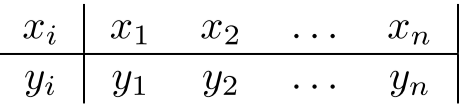
\includegraphics[width=200px]{img/LineareAusgleichsproblemeWertetabelle.png}
	\captionof{figure}{Ausgehende Wertetabelle von linearen Ausgleichsprobleme}
	\label{fig:Ausgehende Wertetabelle von linearen Ausgleichsprobleme}
\end{Figure}

suchen wir die Ausgleichsgerade der Form $f(x)=ax+b$, also $F:=\{a_1f_1 + a_2f_2 | a_1, a_2 \in \mathbb{R}\}$ mit den Ansatzfunktionen $f_1(x) = x$ und $f_2(x) = 1$\\
Das Fehlerfunktional hat dann die Form
\begin{equation}
	E(f)(a,b) := E(f) = \sum\limits_{i=1}^n (y_i - f(x_i))^2 = \sum\limits_{i=1}^n (y_i - (ax_i + b))^2
\end{equation}
Dieses soll minimal werden, d.h. die partiellen Ableitungen nach den Parametern \textit{a} und \textit{b} müssen verschwinden (in Analogie zum eindimensionalen Fall):
\begin{Figure}
\centering
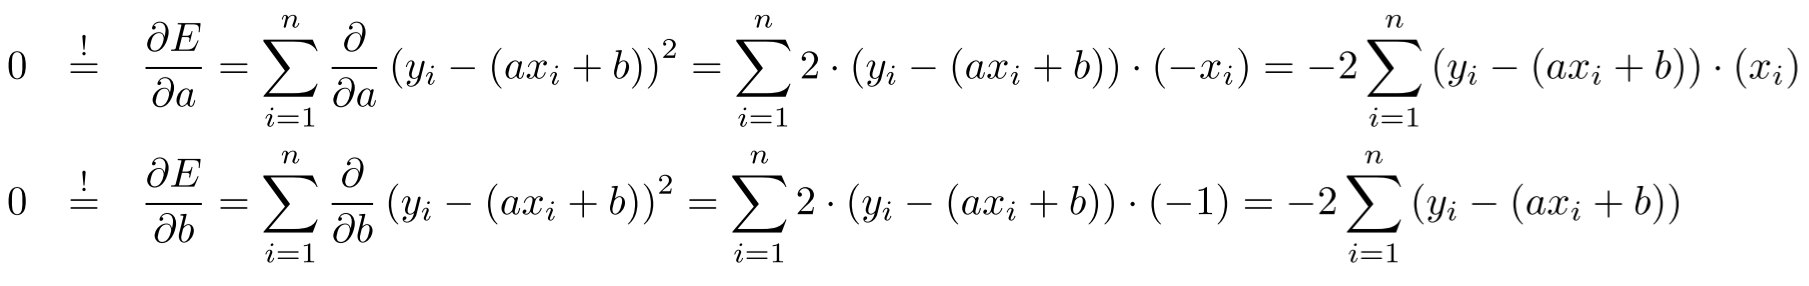
\includegraphics[width=400px]{img/partielleAbleitungAundB.png}
	\captionof{figure}{partielle Ableitung von a und b}
	\label{fig:partielle Ableitung von a und b}
\end{Figure}
Wir haben also zwei Gleichungen für die Unbekannten \textit{a,b}. Durch die Umformung erhalten wir
\begin{Figure}
\centering
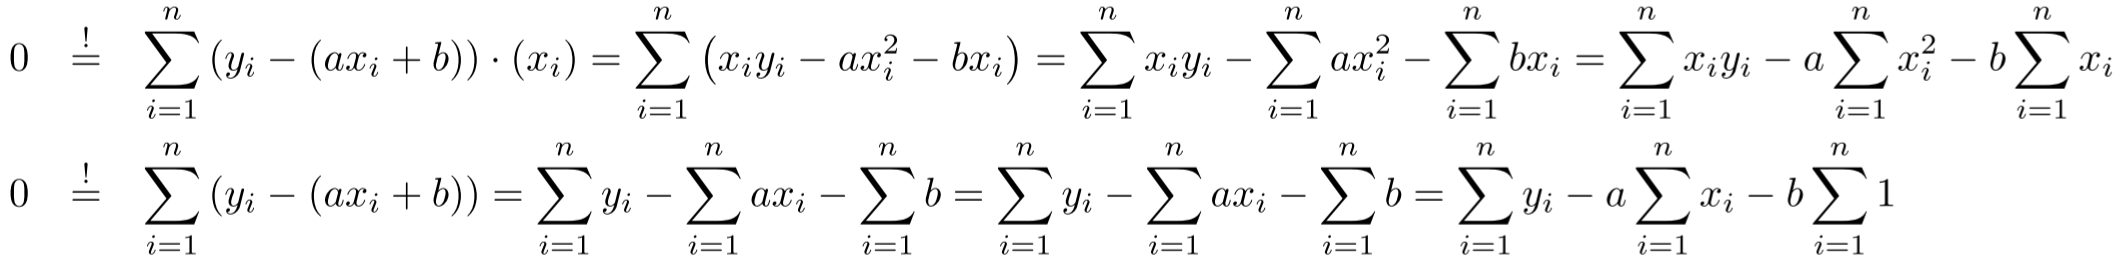
\includegraphics[width=400px]{img/partielleAbleitungAundBUmformung.png}
	\captionof{figure}{Umformung der partiellen Ableitung von a und b}
	\label{fig:Umformung der partiellen Ableitung von a und b}
\end{Figure}
Daraus folgt:
\begin{equation}
\begin{split}
a \sum\limits_{i=1}^n x^2_i + b \sum\limits_{i=1}^n x_i &= \sum\limits_{i=1}^n x_iy_i\\
a \sum\limits_{i=1}^n x_i + \underbrace{b \sum\limits_{i=1}^n 1}_{\substack{n}} &= \sum\limits_{i=1}^n y_i
\end{split}
\end{equation}
oder in der Matrixschreibweise erhalten wir das lineare Gleichungssystem für die Unbekannten (a,b) und können dieses nach \textit{a,b} auflösen
\begin{Figure}
\centering
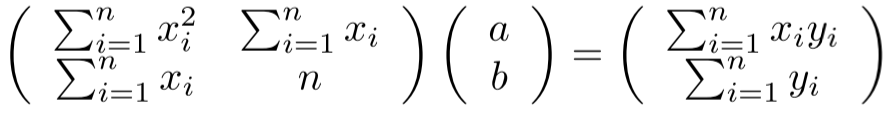
\includegraphics[width=200px]{img/LineareAusgleichsproblemeMatrix.png}
	\captionof{figure}{Matrixschreibweise von linearen Ausgleichsprobleme}
	\label{fig:Matrixschreibweise von linearen Ausgleichsprobleme}
\end{Figure}

\theoremstyle{definition}
\begin{tcolorbox}
\begin{definition}[\textbf{lineares Ausgleichsproblem}]
Gegeben seien \textit{n} Wertepaare ($x_i, y_i$),$i = 1, ..., n$ und \textit{m} Basisfunktionen $f_1, ..., f_m$ auf einem Intervall \[a,b\]. Wir wählen F als die Menge der Ansatzfunktionen $f:= \lambda_1 f_1 + ... + \lambda_m f_m$ mit $\lambda_j \in \mathbb{R}$ also $ F=\{f = \lambda_1 f_1 + ... + \lambda_m f_m | \lambda_j \in \mathbb{R}, j = 1, ..., m\}$\\
Es liegt dann ein \textbf{lineares Ausgleichsproblem} vor mit dem Fehlerfunktional
\begin{equation}
	\begin{split}
	E(f) &= || y - f(x) ||^2_2 \\
		&= \sum\limits_{i=1}^n (y_i - f(x_i))^2 \\
		&= \sum\limits_{i=1}^n (y_i - \sum\limits_{i=1}^m \lambda_j f_j (x_i))^2 \\
		&= || y - A \lambda||^2_2
\end{split}
\end{equation}
vor, wobei
\begin{Figure}
\centering
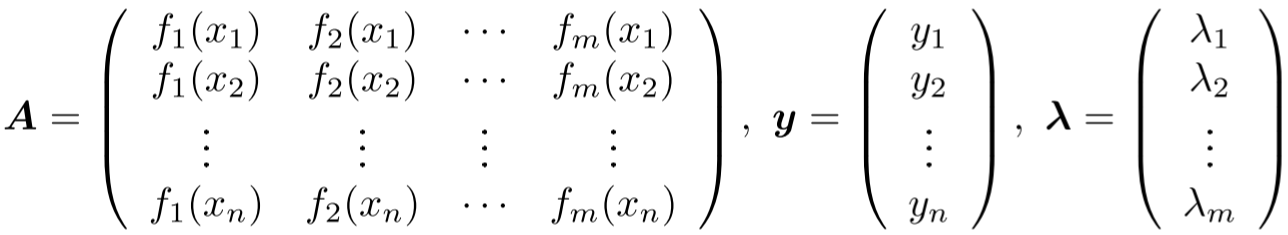
\includegraphics[width=200px]{img/LineareAusgleichsproblemeDefinitionMatrix.png}
	\captionof{figure}{Matrixschreibweise}
	\label{fig:Matrixschreibweise}
\end{Figure}
$\rightarrow$ Das System $A \lambda = y$ heisst \textbf{Fehlergleichungssystem}\\
\textbf{Bemerkungen: }
\begin{itemize}
	\item Das Fehlergleichungssystem besitzt \textit{n} Gleichungen mit \textit{m} Unbekannte. In der Regel ist $n>m$, dementsprechend haben wir mehr Gleichungen als Unbekannt $\rightarrow$ das LGS ist überbestimmt. Man kann daher nicht damit rechnen, dass es eine Lösung gibt
	\item Für $m=n$ haben wir eine eindeutige Lösung und $E(f) = 0$. Dies ist gleichbedeutend damit, dass die Ausgleichsfunktion f exakt durch sämtliche Wertepaare geht. Dies ist ein Spezialfall der Interpolation
\end{itemize}
\end{definition}
\end{tcolorbox}


\theoremstyle{definition}
\begin{tcolorbox}
\begin{definition}[\textbf{Normalgleichungen / Normalgleichungssystem}]
Die Gleichungen
\begin{equation}
\frac{\varphi E(f)(\lambda_1, ..., \lambda_m)}{\varphi \lambda_j} = 0 \quad j = 1, ..., m
\end{equation}
heissen \textbf{Normalgleichungen} des linearen Ausgleichsproblems\\
Das System sämtlicher Normalgleichungen heisst \textbf{Normalgleichugnssystem} und lässt sich als lineares Gleichungssystem schreiben
\begin{equation}
	A^T A \lambda = A^T y
\end{equation}
\textbf{Bemerkungen: }\\
Die Lösungen des Normalgleichungssystem sind die gesuchten Parameter des linearen Ausgleichproblems. Die m x m Matrix \textbf{A}$^T$ \textbf{A} ist symmetrisch und positiv definit, das Normalgleichungssystem kann deshalb mit der  Cholesky-Zerlegung gelöst werden. Numerisch stabiler ist die sogenannte QR-Zerlegung.
\end{definition}
\end{tcolorbox}

\subsection{Nichtlineare Ausgleichsprobleme}
Wir haben gesehen, dass es die Möglichkeit gibt ein nichtlineares Ausgleichsproblem in ein lineares Ausgleichsproblem umzuwandeln. Jedoch soll man in der Lage sein ein nichtlineares Ausgleichsproblem enstprechend lösen zu können.

\theoremstyle{definition}
\begin{tcolorbox}
\begin{definition}[\textbf{Allgemeines Ausgleichsproblem}]
Gegeben seien \textit{n} Wertepaare ($x_i,y_i$), i = 1, ..., \textit{n}, und die Menge F der Ansatzfunktionen $f_p = f_p (\lambda_1, \lambda_2, ..., \lambda_m, x)$ mit \textit{m} Parametern $\lambda_j \in \mathbb{R}$, j = 1, ..., m also $F=\{f_p(\lambda_1, \lambda_2, ..., \lambda_m, x) | \lambda_j \in \mathbb{R}, j = 1, ..., m\}$\\
Das \textbf{allgemeine Ausgleichproblem} besteht darin, die m Parameter $\lambda_1, ..., \lambda_m$ zu bestimmen, so dass das Fehlerfunktional E
\begin{equation}
\begin{split}
E(f) &= \sum\limits_{i=1}^n (y_i - f_p (\lambda_1, \lambda_2, ..., \lambda_m, x_i))^2\\
&= || \begin{pmatrix}
y_1 - f_p(\lambda_1, \lambda_2, ..., \lambda_m, x_1)\\
y_2 - f_p(\lambda_1, \lambda_2, ..., \lambda_m, x_2)
.\\
.\\
.\\
y_n - f_p(\lambda_1, \lambda_2, ..., \lambda_m, x_n)
\end{pmatrix} ||^2_2\\
&= || y - f(\lambda)||^2_2
\end{split}
\end{equation}
minimal wird unter allen zulässigen Parameterbelgungen, wobei
\begin{Figure}
\centering
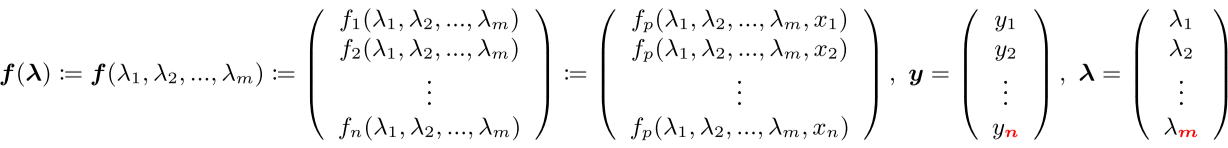
\includegraphics[width=400px]{img/AllgAusgleichsproblemBedingungen.png}
	\captionof{figure}{Bedingungen bei allgemeinen Ausgleichsproblem}
	\label{fig:Bedingungen bei allgemeinen Ausgleichsproblem}
\end{Figure}
\textbf{Bemerkungen: }\\
\begin{itemize}
	\item Falls die Ansatzfunktion $f_p$ linear in den Paramtern sind, haben wir den Spezialfall des linearen Ausgleichsproblems mit $f(\lambda) = A\lambda$
	\item {Das allg. Ausgleichproblem ist also äquivalent zur Bestimmung des Minimums einer Funktion 
	\begin{equation}
	E: \mathbb{R}^m \rightarrow \mathbb{R}
	\end{equation}
	und wir könnten wieder die Normalgleichungen aufstellen, indem wir die partiellen Ableitungen von f nach den Paramtern $\lambda_i$ gleich Null setzen und das etnstehnde, diesmal nicht lineare Gleichungssystem lösen.
	}
\end{itemize}
\end{definition}
\end{tcolorbox}

\subsection{Das Gauss-Newton-Verfahren}

\theoremstyle{definition}
\begin{tcolorbox}
\begin{definition}[\textbf{Quadratmittelproblem}]
Gegeben ist eine Funktion $g: \mathbb{R}^m \rightarrow \mathbb{R}^n$ und das zugehörige Fehlerfunktional $E: \mathbb{R}^m \rightarrow \mathbb{R}$, definiert durch 
\begin{equation}
	E(\textbf{x}) :) || \textbf{g(x)} ||^2_2
\end{equation}
Das Problem, einen Vektor $\textbf{x} \in \mathbb{R}^m$ zu finden, für den E(\textbf{x}) minimal wird, nennt man \textbf{Quadratmittelproblem}
\end{definition}
\end{tcolorbox}

\textbf{evtl. Seite 153 ergänzen?!}


\theoremstyle{definition}
\begin{tcolorbox}
\begin{definition}[\textbf{Gauss-Newton-Verfahren}]
Sei $\lambda^{(0)}$ ein Startvektor in der Nähe des Minimums von E.Das Gauss-Newton-Verfahren zur näherungsweisen Bestimmung des Minimums lautet für k = 0, 1, ...:
\begin{enumerate}
	\item {Berechne $\delta^{(k)}$ als Lösungs des linearen Ausgleichsproblems
		\begin{equation}
		min || g(\lambda^{(k)}) + Dg(\lambda^{(k)})*\delta^{(k)}||^2_2
		\end{equation}			
	d.h. löse konkret:
		\begin{equation}
		Dg(\lambda^{(k)})^T Dg(\lambda^{(k)}) \delta^{(k)} = -Dg(\lambda^{(k)})^T*g(\lambda^{(k)})
		\end{equation}
		nach $\delta^{(k)}$ auf
	}
	\item {Setze
	\begin{equation}
	\lambda^{(k+1)} = \lambda^{(k)} + \delta^{(k)}
	\end{equation}
	}
\end{enumerate}
\end{definition}
\end{tcolorbox}

\theoremstyle{definition}
\begin{tcolorbox}
\begin{definition}[\textbf{gedämpftes Gauss-Newton-Verfahren}]
Sei \textbf{$\lambda^{(0)}$} ein Startvektor in der Nähe des Minimums von E. Das gedämpfte Gauss-Newton-Verfahren zur näherungsweisen Bestimmung des Minimums für k = 0,1,... lautet:
\begin{enumerate}
	\item {Berechne $\sigma^{(k)}$ als Lösung des linearen Ausgleichsproblems
	\begin{equation}
		min || g(\lambda^{(k)}) + Dg(\lambda^{(k)})*\delta^{(k)}||^2_2
	\end{equation}
	d.h. als Lösung des linearen Gleichungssystems
	\begin{equation}
		Dg(\lambda^{(k)})^T Dg(\lambda^{(k)} \delta^{(k)} = -Dg(\lambda^{(k)})^T * g(\lambda^{(k)})
	\end{equation}
	nach $\lambda^{(k)}$ auf
	}
	\item { Finde das minimale $p \in \{0, 1, ..., p_{max}\}$ mit
	\begin{equation}
		||g \underbrace{(\lambda^{(k)} + \frac{\delta^{(k)}}{2^p})}_{\substack{\lambda^{k+1}}} ||^2_2 < || g(\lambda^{(k)})||^2_2
	\end{equation}
	}
	\item Falls kein minimales $p$ gefunden werden kann, rechne mit $p=0$ weiter
	\item {Setze
	\begin{equation}
		\lambda^{(k+1)} = \lambda^{(k)} + \frac{\delta^{(k)}}{2^P}
	\end{equation}
	}
\end{enumerate}
\textbf{Bemerkungen: }\\
\begin{itemize}
	\item Ein Vorteil ist, dass es in der Regel für einen grösseren Bereich von Startvektoren konvergiert als das ungedämpfte Gaus-Newton-Verfahren. Durch das fortlaufende Anpassen der "Korrekturrichtung" kann es sozusagen noch mit Startvektoren umgehen, die weiter entfernt sind vom Optimum. Die Dämpfung ist aber keine Garantie für Konvergenz. Man benötigt noch weitere Bedingungen. 
	\item {Als Abbruchkriterium des Algorithmus kann z.B. 
	\begin{equation}
		|| \frac{\delta^{(k)}}{2^P}||_2 TOL
	\end{equation}
	verwendet werden. Wiederum ist das aber keine Garantie, dass die berechnete Näherung einen maximalen ABstand von TOL zum gesuchten Minimum besitzt
	}
\end{itemize}
\end{definition}
\end{tcolorbox}


\section{Fourier-Reihen und Fourier-Transformation}
Die Theorie der Fourier-Reihen und Fourier-Transformation ermöglicht die Zerlegung eines periodischen Signals in eine unendliche Summe (d.h. Reihe) von harmonischen Schwingungen der Form $A cos(\omega t + \phi)$ oder $B sin(\omega t + \phi)$

\subsection{Lernziele}
\begin{itemize}
	\item Sie kennen wichtige Anwendungsfälle der Fourier-Theorie
	\item Sie kennen die Definition einer Fourier-Reihe und können deren Koeffizienten berechnen
	\item Sie können die diskrete Fourier-Transformation auf konkrete Problemstellung anwenden und in MATLAB implementieren
\end{itemize}

\subsection{Anwendungen}
Es macht möglich, ein beliebiges Signal (z.B. in Form einer Schall- oder elektromagnetischen Welle) in seine Frequenzen zu zerlegen bzw. aus einem Frequenzspektrum des ursprünglichen Signal zu rekonstruieren. Was die Fourier-Analyse so einzigartig macht, ist die Möglichkeit, sie unmittelbar physikalisch zu erfahren. \\
Mögliche Anwendungsgebiete:\\
\begin{itemize}
	\item Detektion von Frequenzen
	\item Entrauschen von verrauschten Signalen
	\item MP3-Verfahren zur Komprimierung von Audiodateien
	\item Bildverarbeitung bspw. JPEG
\end{itemize}

\subsection{Fourier-Reihen}
\textbf{Evtl. Seiten 162-164 ergänzen}

\subsubsection{Allgemeine Fourier-Reihen}

\theoremstyle{satz}
\begin{tcolorbox}
\begin{satz}[Fourier-Reihen / Fourier-Koeffizienten]
Sei $f: \mathbb{R} \rightarrow \mathbb{R}$ eine periodische Funktion mit der Kreisfrequenz $\omega_0$ und Periode $T = \frac{2 \pi}{\omega_0}$. Des Weiteren lasse sich das Periodenintervall in endlich viele Teilintervalle zerlegen, in denen $f(x)$ stetig und monoton ist, und in den Unstetigkeitsstellen existiere sowohl der links- als auch der rechtsseitge Grenzwert (Dirichletschte Bedingungen).\\
Dann kann $f(x)$ in eine \textbf{Fourier-Reihe} der Form
\begin{equation}
	f(x) = \frac{A_0}{2} + \sum\limits^{\infty}_{k=1} [A_k cos (k * \omega_0 * x) + B_k sin(k * \omega_0 * x)]
\end{equation}
entwickelt werden. Dabei bedeuten:\\
\begin{itemize}
	\item[-] $\omega_0 = \frac{2 \pi}{T}$: Kreisfrequenz der Grundschwingung
	\item[-] $k * \omega_0$: Kreisfrequenz der sogenannten k-ten harmonischen Oberschwingung
\end{itemize}

Die \textbf{Fourierkoeffizienten} von f werden dabei aus den Integralformeln
\begin{equation}
\begin{split}
	A_0 &= \frac{2}{T} \int_{(T)} f(x) dx\\
	A_k &= \frac{2}{T} \int_{(T)} f(x) cos(k \omega_0 x) dx\\
	B_k &= \frac{2}{T} \int_{(T)} f(x) sin(k \omega_0 x) dx
\end{split}
\end{equation}
berechnet. Das Symbol (T) unter dem Integral bedeutet, dass die Integration über ein beliebiges Intervall der Länge T zu erstrecken ist.\\
Die \textbf{Amplitude} des k-ten Fourierkoeffizienten berechnet sich zu
\begin{equation}
\begin{split}
	amp_{k=0} &:= \frac{A_0}{2}\\
	amp_k &:= \sqrt{A^2_k + B^2_k}
\end{split}
\end{equation}
\end{satz}
\end{tcolorbox}

\subsection{diskrete Fourier-Transformation}
Bisher war die Funktion $f(x)$ in analytischer Form gegeben. Tatsächlich findet man in vielen Anwendungen mit einer endlichen Anzahl von diskreten Datenpunkten (bspw. Messungen, Bilder, Tonaufnahme etc.). Hier befassen wir uns mit FOurier-Reihen für Funktionen mit \textbf{äquidistanten} Punkten (sprich mit gleichem Abstand zwischen den Datenpunkten

\theoremstyle{satz}
\begin{tcolorbox}
\begin{satz}[Diskrete Fourier-Reihen / Diskrete Fourier-Koeffizienten (DFT)]
 Sei $f: [0,T] \rightarrow \mathbb{R}$ definiert durch $2n+1$ äquidistante Punkte $(t_i, f(t_i))$ mit i = 1, ..., 2n+1 und $f(0) = f(T)$ Der Abstand zwischen den Punkten sei konstant $\Delta t = \frac{T}{2n}$ d.h. $t_i = (i-1) * \Delta t$. Dann kann $f(t_i)$ in eine \textbf{diskrete Fourier-Reihe} der Form
\begin{equation}
 	f(t_i) = \sum\limits^n_{k=0} [A_k cos(k*\omega_0*t_i + B_k sin(k*\omega_0 * t_i)]
\end{equation}
entwickelt werden, auch bekannt als \textbf{inverse reelle diskrete Fourier-Transformation}. Der letzte Punkt mit $t_{2n+1} = T$ wird nicht berücksichtigt, da $f(0) = f(T)$. Dabei bedeuten:\\
\begin{itemize}
	\item[-] $\omega_0 = \frac{2 \pi}{T}$: Kreisfrequenz der Grundschwingung
	\item[-] $k * \omega_0$: Kreisfrequenz der sogenannten k-ten harmonischen Oberschwingung
\end{itemize}
Die \textbf{diskreten Fourierkoeffizienten} von $f$ werden dabei aus
\begin{equation}
\begin{split}
	A_0 &= \frac{1}{2n} \sum\limits_{i=1}^{2n} f(t_i)\\
	A_k &= \frac{1}{n} \sum\limits_{i=1}^{2n} f(t_i) cos(k * \omega_0 * t_i) \quad k=1,2,...,n-1\\
	A_n &= \frac{1}{2n} \sum\limits_{i=1}^{2n} f(t_i) cos(n * \omega_0 * t_i)
\end{split}
\end{equation}
und
\begin{equation}
\begin{split}
	B_0 &= 0 \\
	B_k &= \frac{1}{n} \sum\limits_{i=1}^{2n} f(t_i) sin(k * \omega_0 * t_i) \quad k=1,2,...,n-1\\
	B_n &= 0
\end{split}
\end{equation}
berechnet. Die Koeffizienten $A_k$ und $B_k$ werden auch \textbf{reelle diskrete Fourier-Transformation} genannt.\\
\textbf{Bemerkungen: }\\
\begin{itemize}
	\item Die Koeffizienten $A_k$ und $B_k$ beschreiben die Funktion $f(t)$ im Frequenzbereich. Sie erlauben, die Funktion quasi aus der Zeit- (oder Orts-) Domäne in die Frequenzdomäne zu transformieren, deshalb der Begriff "Diskrete Fourier-Transformation"
	\item {Die Rücktransformation aus der Frequenzdomäne i ndie Zeit- (oder Orts-) Domäne erfolgt über $f(t_i) = \sum\limits^n_{k=0} [A_k cos(k * \omega_0 * t_i) + B_k sin(k * \omega_0 * t_i)]$ deshalb der Begriff \dq inverse diskrete Foruier-Transformation\dq
	\begin{equation}
		\{f(t_1), f(t_2), ..., f(t_{2n}\} \stackrel{DFT}\rightarrow \{A_0, A_1, ..., A_n, B_0, B_1, ..., B_n\} \stackrel{inverse DFT}\rightarrow \{f(t_1), f(t_2), ..., f(t_2n)\}
	\end{equation}		
	}
	\item Falls $f(0) \neq f(T)$, ersetzt man üblicherweise $f(0)$ und $f(T)$ mit $\frac{f(0)+f(T)}{2}$
	\item die reelle DFT ist von der Ordnung $O(n^2)$. Für grosse n gibt es den schnelelren Algorithmus der "Fast Fouriert Transform" welcher die Ordnung $O(n\ log\ n)$ hat. In MATLAB gibt es dazu die Funktion "fft.m"
\end{itemize}
\end{satz}
\end{tcolorbox}

Eine einfache Art, das Frequenzspektrum grafisch darzustellen, ist das sogenannte Leistungsdichte-Spektrum. Handelt es sich beim Signal $f(t)$ um eine elektromagnetische Welle, entspricht das Quadrat der Fourierkoeffizienten der Energie dieser Welle bei der k-ten Frequenz. Je mehr Energie (d.h. je grösser das Quadrat der Fourier-Koeffizienten) bei einer spezifischen Frequenz, umso dominanter ist die entsprechende harmonische Schwingung.

\theoremstyle{definition}
\begin{tcolorbox}
\begin{definition}[\textbf{Leistungsdichte-Spektrum / Power-Spektrum}]
Wir definieren das Leistungsdichte-Spektrum / Power-Spektrum für die diskrete Fourier-Transformation als
\begin{equation}
	P_k = \frac{1}{4}\frac{(A^2_k + B^2_k)}{n} \quad k = 0, ..., n
\end{equation}
für die k-te Frequenz $v_k = \frac{k*\omega_0}{2 \pi} = \frac{k}{T}$
\end{definition}
\end{tcolorbox}



\end{document}
